
\documentclass[12pt, a4paper, oneside]{book}
\usepackage{listings}
\usepackage{color} 
\lstset{
    inputencoding=utf8,         % <-- MUY IMPORTANTE
    extendedchars=true,         % <-- Activar caracteres extendidos (acentos, ñ, etc.)
    literate=%
        {á}{{\'a}}1 {é}{{\'e}}1 {í}{{\'i}}1 {ó}{{\'o}}1 {ú}{{\'u}}1
        {Á}{{\'A}}1 {É}{{\'E}}1 {Í}{{\'I}}1 {Ó}{{\'O}}1 {Ú}{{\'U}}1
        {ñ}{{\~n}}1 {Ñ}{{\~N}}1
        {¿}{{?}}1 {¡}{{!}}1,
    breaklines=true,
    breakatwhitespace=true,
    columns=flexible,
    basicstyle=\ttfamily\small,
    numbers=left,
    numberstyle=\tiny\color{gray},
    frame=single,
    captionpos=b,
    keepspaces=true,
    tabsize=4,
}
\usepackage{tikz}
\usetikzlibrary{shapes,arrows,positioning}
\usepackage[spanish]{babel}
\usepackage[utf8]{inputenc}
\usepackage[T1]{fontenc}
\usepackage{geometry}
\geometry{a4paper, margin=2.5cm}

\usepackage{titlesec}
\usepackage{titletoc}
\usepackage{hyperref}
\usepackage{graphicx}
\usepackage{tabularx}
\usepackage{xcolor}
\usepackage{amsmath}
\usepackage{natbib}
\usepackage{appendix}

\hypersetup{
    colorlinks=true,
    linkcolor=blue,
    filecolor=magenta,      
    urlcolor=cyan,
    pdftitle={TFG Pablo Moreno Muñoz},
}

\titleformat{\chapter}[display]
{\normalfont\bfseries\Huge}{\chaptertitlename\ \thechapter}{20pt}{\Huge}
\titlespacing*{\chapter}{0pt}{-30pt}{40pt}

\setcounter{secnumdepth}{3}
\setcounter{tocdepth}{3}

\begin{document}

\begin{titlepage}
    \centering
    \vspace*{2cm}
    {\LARGE Universidad de Zaragoza \par}
    \vspace{1cm}
    {\Huge\bfseries Diseño e implementación de un sistema basado en wearables Fitbit para el monitoreo de la salud de personas mayores \par}
    \vspace{2cm}
    {\Large Pablo Moreno Muñoz \par}
    \vspace{1cm}
    {\large Trabajo Fin de Grado \par}
    \vspace{1cm}
    {\large Grado en Ingeniería Informática \par}
    \vspace{1cm}
    {\large Directores: Raquel Trillo y Laura Po \par}
    \vspace{2cm}
    {\large \today \par}
\end{titlepage}

\chapter*{Resumen}
 Este trabajo se enmarca en la creciente necesidad de soluciones tecnológicas para la atención sanitaria de la población anciana. Presentamos el diseño y la implementación de un sistema de monitorización remota de salud, apoyado en dispositivos Fitbit, que permite el seguimiento continuo de indicadores como la frecuencia cardíaca, los niveles de actividad física y la calidad del sueño.

El sistema desarrollado emplea un backend modular basado en microservicios, diseñado con criterios de escalabilidad y resiliencia. Se integra de manera segura con la API de Fitbit utilizando el protocolo OAuth 2.0, y permite la adquisición y almacenamiento eficiente de datos en bases de datos especializadas en series temporales.  Además, se incorpora un pipeline que procesa los datos de forma automatizada tras su recepción, permitiendo la detección de eventos críticos, y paneles visuales accesibles e intuitivos que permiten a cuidadores o profesionales de la salud visualizar la evolución del estado de los usuarios de forma clara.

La tesis expone los requerimientos técnicos, las decisiones arquitectónicas adoptadas, los desafíos enfrentados y las pruebas realizadas para validar el sistema. Asimismo, se analizan las implicaciones éticas y legales relacionadas con el tratamiento de datos personales de salud, cumpliendo con el Reglamento General de Protección de Datos (RGPD). Finalmente, se discuten las oportunidades de mejora y expansión del sistema, incluyendo la integración con nuevas plataformas de dispositivos vestibles y el uso de técnicas de inteligencia artificial para predicción de eventos adversos.

\vspace{1cm} % Espacio opcional
\textbf{Palabras clave:} Monitorización remota, Fitbit, Salud ancianos, OAuth 2.0. 

\tableofcontents

% -*- coding: utf-8 -*- % Para asegurar codificación correcta
\chapter{Introducción}
\label{chap:introduccion}
A continuación se introduce el contexto y la motivación de este proyecto, para luego definir sus objetivos, alcance y la organización general de este documento
\section{Contexto y Motivación}
\label{sec:intro_contexto}

El envejecimiento de la población es una realidad demográfica global, especialmente acentuada en España, donde, según el Instituto Nacional de Estadística, más del 20\% de la población tiene más de 65 años y se prevé que esta cifra siga aumentando en las próximas décadas \cite{ine_proyeccion_2022_2072}. Este fenómeno implica un incremento en la prevalencia de enfermedades crónicas y una mayor demanda de servicios sanitarios y de cuidados de larga duración, lo que genera una presión significativa sobre los sistemas de salud y las familias \cite{who_ageing_health}. En este escenario, la tecnología emerge como un aliado fundamental para desarrollar soluciones innovadoras que mejoren la calidad de vida de las personas mayores, promuevan su autonomía y faciliten su cuidado.

La monitorización remota de la salud, apoyada en dispositivos electrónicos y sensores, ofrece un enorme potencial para el seguimiento continuo y no invasivo de indicadores fisiológicos y de actividad \cite{majumder2017wearable}. Los dispositivos vestibles o \textit{wearables}, como las pulseras de actividad y los relojes inteligentes, se han popularizado enormemente en los últimos años. Entre ellos, Fitbit\textsuperscript{\textregistered} destaca por su amplia adopción, facilidad de integración mediante API y coste accesible, lo que lo convierte en una opción idónea para proyectos de monitorización remota.

La motivación principal de este Trabajo Fin de Grado (TFG) radica en explorar y aprovechar el potencial de estos dispositivos comerciales, específicamente los de Fitbit\textsuperscript{\textregistered}, para construir un sistema que facilite la monitorización remota de personas mayores por parte de sus cuidadores o personal sanitario. El objetivo es contribuir a una atención más proactiva, permitiendo detectar posibles cambios en el estado de salud de forma temprana y mejorando la tranquilidad de los familiares y responsables del cuidado, respetando la autonomía y privacidad del usuario monitorizado.

\section{Definición del Problema}
\label{sec:intro_problema}

A pesar de la disponibilidad de datos generados por dispositivos como Fitbit\textsuperscript{\textregistered}, a menudo existe una brecha entre la simple recolección de datos y su utilización efectiva para el seguimiento de la salud, especialmente en el contexto de personas mayores y sus cuidadores. Los problemas específicos que este trabajo busca abordar son:

\begin{itemize}
    \item La falta de sistemas integrados que recopilen automáticamente datos relevantes de Fitbit\textsuperscript{\textregistered} y los presenten de forma clara, contextualizada y comprensible para cuidadores no necesariamente expertos en tecnología.
    \item La dificultad para realizar un seguimiento longitudinal de los indicadores clave de salud obtenidos a través de estos dispositivos, identificando tendencias o desviaciones significativas de los patrones habituales del usuario.
    \item La necesidad de implementar soluciones técnicas robustas que gestionen de forma segura la autenticación con servicios de terceros (Fitbit API) y que respeten escrupulosamente la privacidad y la normativa de protección de datos (como el RGPD) al manejar información personal y sensible de salud.
    \item La ausencia frecuente de arquitecturas flexibles y escalables en prototipos de este tipo, que permitan una futura expansión para incluir más usuarios, más tipos de datos o integración con otros sistemas.
\end{itemize}

Este TFG se enfoca en el diseño e implementación de un prototipo que dé respuesta a estos desafíos, proporcionando una solución técnica robusta, funcional y bien documentada.

\section{Objetivos}
\label{sec:intro_objetivos}

Para abordar el problema definido, se establecen los siguientes objetivos, diferenciando entre el objetivo general y los específicos:

\subsection{Objetivo General}
\label{subsec:obj_general}

Diseñar e implementar un prototipo de sistema software para la monitorización remota de indicadores de salud de personas mayores, utilizando datos obtenidos de pulseras de actividad Fitbit\textsuperscript{\textregistered} y presentando la información de forma útil y accesible para cuidadores o personal autorizado, con un enfoque en la seguridad, la privacidad y la escalabilidad.

\subsection{Objetivos Específicos}
\label{subsec:obj_especificos}

\begin{enumerate}
    \item Investigar en profundidad la API web de Fitbit\textsuperscript{\textregistered}, su modelo de datos, las políticas de acceso, la granularidad de los datos disponibles y el proceso de autorización seguro mediante OAuth 2.0.
    \item Diseñar una arquitectura software para el backend del sistema, basada en microservicios ligeros implementados en Python (Flask), que sea modular y escalable.
    \item Implementar un microservicio responsable de gestionar la autenticación de los usuarios del sistema (cuidadores, administradores) y la obtención segura de tokens de acceso para la API de Fitbit\textsuperscript{\textregistered} mediante el flujo OAuth 2.0.
    \item Desarrollar un microservicio encargado de la adquisición periódica y automatizada de los datos de interés de los usuarios desde la API de Fitbit\textsuperscript{\textregistered} (frecuencia cardíaca diaria/intradía, resumen del sueño, pasos y niveles de actividad).
    \item Seleccionar, configurar e implementar una base de datos relacional PostgreSQL con extensión TimescaleDB, adecuada para el almacenamiento eficiente y la consulta de los datos biométricos y de actividad a lo largo del tiempo.
    \item Implementar la lógica necesaria para el procesamiento básico de los datos adquiridos, incluyendo la validación, limpieza y transformación de los datos para su almacenamiento y posterior visualización (cálculo de promedios, identificación de periodos de inactividad/actividad).
    \item Desarrollar un panel de visualización web (dashboard) sencillo e intuitivo utilizando Flask y plantillas HTML, que permita a los cuidadores consultar el histórico de datos mediante gráficos interactivos y visualizar indicadores clave.
    \item Definir e implementar un conjunto inicial de criterios basados en evidencia para la detección temprana de posibles anomalías en los datos de actividad, sueño y frecuencia cardíaca, generando alertas contextualizadas para el personal autorizado.
    \item Analizar y aplicar las medidas técnicas y organizativas necesarias para garantizar la seguridad (autenticación, autorización, protección contra ataques comunes) y privacidad de los datos (minimización, seudonimización si aplica, gestión de consentimientos), en cumplimiento con los principios del Reglamento General de Protección de Datos (RGPD).
    \item Validar el correcto funcionamiento del prototipo desarrollado mediante un conjunto definido de pruebas funcionales (cobertura de requisitos), de integración (comunicación entre microservicios y con API externa) y del sistema (flujos de usuario principales).
\end{enumerate}

\section{Alcance y Limitaciones}
\label{sec:intro_alcance}

El sistema desarrollado en este TFG es un prototipo funcional que demuestra la viabilidad técnica de la solución propuesta. El alcance del trabajo cubre:

\begin{itemize}
    \item Integración con la API de Fitbit\textsuperscript{\textregistered} para obtener datos de frecuencia cardíaca (resumen diario y/o intradía según disponibilidad de la API), patrones de sueño (fases, duración) y actividad física (pasos, minutos activos).
    \item Desarrollo de un backend modular basado en microservicios ligeros implementados en Python (Flask).
    \item Almacenamiento de los datos en una base de datos relacional PostgreSQL con TimescaleDB.
    \item Implementación completa del flujo de autenticación OAuth 2.0 con Fitbit\textsuperscript{\textregistered} para la autorización segura por parte del usuario.
    \item Desarrollo de una interfaz web básica para cuidadores, que permite visualizar gráficos históricos de los datos y gestionar usuarios monitorizados.
    \item Implementación de lógica para evaluar criterios de alerta predefinidos sobre los datos de actividad, sueño y frecuencia cardíaca.
    \item Aplicación de principios de diseño orientados a la seguridad y al cumplimiento del RGPD (por ejemplo, cifrado de datos sensibles en reposo y en tránsito, gestión segura de tokens).
\end{itemize}

Es importante destacar las siguientes limitaciones:

\begin{itemize}
    \item El sistema \textbf{no es un dispositivo médico certificado} y la información proporcionada no debe utilizarse para autodiagnóstico ni para sustituir la consulta con un profesional sanitario cualificado. Su propósito es informativo y de apoyo al cuidado.
    \item La funcionalidad está limitada a los datos y la granularidad que Fitbit\textsuperscript{\textregistered} expone a través de su API web estándar (por ejemplo, la frecuencia cardíaca intradía puede estar limitada a intervalos de 1 minuto o más, dependiendo del nivel de acceso a la API).
    \item El sistema de alertas implementado se basa en criterios iniciales y no incluye mecanismos avanzados de inteligencia artificial para predicción o adaptación dinámica de umbrales. La validación clínica de las alertas generadas queda fuera del alcance de este prototipo.
    \item El prototipo ha sido validado funcionalmente en un entorno de desarrollo y pruebas, pero no ha sido sometido a pruebas de carga extensivas ni a una evaluación de usabilidad formal con usuarios finales (personas mayores y cuidadores).
    \item La interfaz de usuario, aunque funcional, representa un diseño básico y podría beneficiarse de mejoras significativas en términos de experiencia de usuario (UX) y diseño de interfaz (UI) para una adopción real.
    \item El análisis de cumplimiento del RGPD se basa en los principios de diseño y buenas prácticas, pero no constituye una auditoría legal completa ni garantiza la conformidad total en un entorno de producción sin revisiones adicionales.
    \item El sistema no incluye mecanismos avanzados de detección de anomalías o predicción basados en inteligencia artificial, aunque la arquitectura sentaría las bases para su futura integración.
\end{itemize}

\section{Estructura del Documento}
\label{sec:intro_estructura}

La memoria se organiza en los siguientes capítulos:

\begin{itemize}
    \item \textbf{Capítulo 1: Introducción.} (Este capítulo) Presenta el contexto, la motivación, el problema a resolver, los objetivos, el alcance y la estructura del documento.
    \item \textbf{Capítulo 2: Estado del Arte y Marco Tecnológico.} Revisa soluciones existentes en el ámbito de la monitorización remota de salud con wearables y describe en detalle las tecnologías clave seleccionadas y empleadas en el proyecto (Fitbit API, OAuth 2.0, microservicios, bases de datos de series temporales, etc.).
    \item \textbf{Capítulo 3: Análisis y Metodología.} Detalla los requisitos funcionales (lo que el sistema debe hacer) y no funcionales (atributos de calidad como rendimiento, seguridad, usabilidad) identificados para el sistema, y describe brevemente la metodología de desarrollo seguida (ej. iterativa, basada en prototipos).
    \item \textbf{Capítulo 4: Diseño y Arquitectura del Sistema.} Expone las decisiones de diseño tomadas, presentando la arquitectura general del sistema, el diseño detallado de los microservicios del backend, el esquema de la base de datos, el flujo de datos y la integración con la API externa.
    \item \textbf{Capítulo 5: Implementación.} Describe los detalles concretos de la implementación de los componentes más relevantes del sistema, incluyendo el entorno de desarrollo, las librerías principales utilizadas, fragmentos de código ilustrativos y los desafíos técnicos encontrados y cómo fueron resueltos.
    \item \textbf{Capítulo 6: Pruebas y Validación.} Explica la estrategia de pruebas definida y llevada a cabo (pruebas unitarias, de integración, del sistema) para asegurar la calidad del software y validar que el prototipo cumple con los requisitos especificados.
    \item \textbf{Capítulo 7: Resultados y Discusión.} Presenta el prototipo funcional resultante, mostrando ejemplos de su operación (ej. capturas de pantalla del dashboard) y discute los resultados obtenidos en términos de cumplimiento de objetivos, rendimiento observado y las limitaciones inherentes al sistema desarrollado.
    \item \textbf{Capítulo 8: Conclusiones y Trabajo Futuro.} Resume las principales conclusiones extraídas del desarrollo del TFG, destacando las contribuciones del trabajo y proponiendo posibles líneas de mejora, expansión y trabajo futuro sobre el sistema desarrollado.
\end{itemize}
% -*- coding: utf-8 -*-
\chapter{Estado del Arte y Marco Tecnológico}
\label{chap:estado_arte}

Este capítulo revisa el estado actual de la monitorización remota de salud en personas mayores, el papel de los dispositivos vestibles como Fitbit\textsuperscript{\textregistered}, y describe las tecnologías clave empleadas en el sistema desarrollado, justificando su elección.

\section{Monitorización Remota de Salud en Personas Mayores}
\label{sec:ea_monitorizacion_remota}

La monitorización remota de pacientes (RPM, por sus siglas en inglés, \textbf{Remote Patient Monitoring}) ha ganado relevancia en los últimos años, impulsada por los avances tecnológicos y la necesidad de modelos de atención sanitaria más eficientes \cite{noah2022mobile}. En personas mayores, la RPM permite la detección temprana de deterioros, la reducción de hospitalizaciones y la mejora de la independencia y la tranquilidad de usuarios y cuidadores \cite{bashshur2018telemedicine}.

Existen diversas aproximaciones a la RPM, desde sistemas basados en sensores ambientales instalados en el hogar hasta el uso de dispositivos médicos específicos o, cada vez más, el aprovechamiento de dispositivos de consumo como smartphones y wearables \cite{majumder2017wearable}. Sin embargo, la implementación exitosa de sistemas RPM para la población mayor también enfrenta desafíos importantes. Entre ellos destacan la usabilidad y aceptación de la tecnología por parte de los usuarios mayores, la gestión de la gran cantidad de datos generados, la necesidad de garantizar la fiabilidad y precisión de los datos, la interoperabilidad entre diferentes dispositivos y sistemas, y la gestión de la privacidad y seguridad de datos de salud altamente sensibles \cite{lee2021challenges}.

\subsection{Bases científicas y enfoque práctico para la detección de alertas}
\label{subsec:bases_alertas}

Más allá de la simple visualización, el valor añadido de la monitorización remota reside en la detección temprana de cambios relevantes en la salud del usuario. En este sistema, la selección de parámetros y la lógica de alerta se fundamentan en la literatura científica, pero se implementan mediante reglas y umbrales explícitos, adaptados a la práctica real y a las limitaciones de los datos disponibles por Fitbit. Los principales parámetros monitorizados son:

\begin{itemize}
    \item \textbf{Actividad física:} Se monitorizan caídas porcentuales significativas respecto a la media semanal individual, siguiendo la evidencia de que reducciones del 30\% o 50\% en la actividad habitual pueden indicar deterioro funcional o riesgo de eventos adversos \cite{rebelo_physical_inactivity_consequences_2020, who_guidelines_2020}. El sistema genera alertas cuando la actividad diaria cae por debajo de estos umbrales, calculados dinámicamente para cada usuario.
    \item \textbf{Sedentarismo:} Se detectan aumentos notables en el tiempo sedentario, comparando el valor diario con la línea base personal. Umbrales del 30\% y 50\% de incremento se emplean para alertas de prioridad media y alta, respectivamente, en línea con estudios recientes \cite{bellettiere_pa_sedentary_aging_women_2017}.
    \item \textbf{Sueño:} Se evalúan cambios en la duración del sueño respecto al patrón habitual del usuario. Variaciones superiores al 30\% (tanto por exceso como por defecto) generan alertas, dado su vínculo con deterioro cognitivo y fragilidad \cite{nsf_older_adult_sleep_2022, westman_sleep_cognition_nordic_2024, pinto_sleep_frailty_review_2025}.
    \item \textbf{Frecuencia cardíaca:} Se monitorizan anomalías en la frecuencia cardíaca en reposo (RHR) y su variabilidad (HRV), comparando los valores diarios con la media y desviación estándar individual. Se generan alertas si se superan umbrales relativos (por ejemplo, más de 2 desviaciones estándar respecto a la media semanal), siguiendo recomendaciones de la literatura \cite{kang_hrv_thresholds_mortality_2021, shaffer_overview_hrv_2017}.
\end{itemize}

Todos los umbrales se documentan y justifican en los anexos técnicos, y se calculan de forma personalizada para cada usuario.

\subsection{Sistemas de alerta en salud digital: enfoque implementado y efectividad}
\label{subsec:sistemas_alerta_comparativa}

La generación de alertas en este sistema se basa en un enfoque de reglas y umbrales explícitos, implementados en el backend (véase \texttt{alert\_rules.py}), por ser la opción más transparente y trazable para entornos clínicos y de cuidado. Este método, ampliamente utilizado en salud digital \cite{alam_alert_systems_review_2019}, permite adaptar fácilmente los criterios a nuevas evidencias o necesidades del usuario. Aunque existen enfoques más complejos (como modelos predictivos o integración de múltiples fuentes), en este TFG se prioriza la robustez, la interpretabilidad y la facilidad de validación.

Las alertas generadas se notifican a los cuidadores a través del panel web, donde pueden consultarse, filtrar por prioridad y marcar como revisadas.

\subsubsection{Efectividad y limitaciones del enfoque}
La efectividad de los sistemas de alerta depende tanto de la calidad de los datos como de la calibración de los umbrales. El sistema implementado busca minimizar la fatiga de alertas mediante la personalización de los umbrales y la priorización de alertas relevantes, pero reconoce limitaciones inherentes: posibles falsas alarmas si los patrones individuales varían mucho, y la imposibilidad de detectar eventos no reflejados en los datos de Fitbit. La validación empírica y la revisión periódica de los umbrales son esenciales para mantener la utilidad clínica del sistema.

\subsubsection{Justificación y validación de umbrales}
La definición de umbrales se basa en la literatura científica y en la experiencia clínica, pero se adapta a la variabilidad interindividual mediante el uso de porcentajes y comparación con la línea base personal. La justificación detallada de cada umbral y ventana temporal utilizada se documenta en los archivos técnicos del proyecto y se aborda en los capítulos de metodología e implementación.

\section{Dispositivos Wearables: El Caso de Fitbit}
\label{sec:ea_fitbit}

El mercado de dispositivos wearables ha experimentado un crecimiento exponencial, ofreciendo una amplia gama de productos capaces de monitorizar diversos parámetros fisiológicos y de actividad \cite{fortune_wearable_market}. Fitbit\textsuperscript{\textregistered} (ahora parte de Google) se ha consolidado como una de las marcas líderes en el segmento de pulseras y relojes de actividad física y bienestar. Sus dispositivos suelen incluir sensores como acelerómetros (para contar pasos y detectar movimiento/sueño) y fotopletismógrafos (PPG) para medir la frecuencia cardíaca \cite{fitbit_how_hr_works}.

Los datos típicamente accesibles a través de la API de Fitbit\textsuperscript{\textregistered} incluyen resúmenes diarios y, en algunos casos, datos intradía (con granularidad variable) de pasos, distancia, calorías quemadas, minutos de actividad, fases y duración del sueño, y frecuencia cardíaca \cite{fitbit_api_reference}. Si bien estos dispositivos no son instrumentos médicos certificados, diversos estudios han evaluado su precisión. Por ejemplo, la medición de la frecuencia cardíaca en reposo suele considerarse razonablemente precisa, aunque puede disminuir durante actividad física intensa. La detección de fases del sueño y el conteo de pasos también muestran una correlación aceptable con métodos de referencia en muchos estudios, aunque existen limitaciones y variabilidad entre dispositivos y condiciones de uso \cite{haghayegh2019accuracy, nelson2016validity}. Es crucial tener en cuenta estas consideraciones al interpretar los datos y diseñar el sistema. La adquisición de Fitbit por Google puede afectar la disponibilidad futura de la API \cite{google_fitbit_acquisition_info}.
\section{Tecnologías Habilitadoras}
\label{sec:ea_tecnologias}

El desarrollo del sistema de monitorización propuesto se apoya en un conjunto de tecnologías clave que se describen a continuación.

\subsection{API de Fitbit y OAuth 2.0}
\label{subsec:ea_fitbit_api_oauth}

El acceso a los datos de los usuarios de Fitbit\textsuperscript{\textregistered} se realiza exclusivamente a través de su API web oficial. Se trata de una API RESTful que utiliza el formato JSON para el intercambio de datos \cite{fitbit_api_reference}. Proporciona diversos \textit{endpoints} para obtener información del perfil del usuario, resúmenes de actividad diaria, datos de series temporales (como frecuencia cardíaca o pasos a lo largo del día con cierta granularidad), información sobre el sueño, etc. Para poder acceder a los datos de un usuario, es imprescindible obtener su consentimiento explícito a través del protocolo de autorización estándar \textbf{OAuth 2.0} \cite{oauth_spec_rfc6749}.

En este proyecto, se implementa el flujo \textit{Authorization Code Grant} de OAuth 2.0, considerado el más seguro para aplicaciones web con backend. Dado que la aplicación web desarrollada está pensada para ser operada por personal autorizado (ej. un recepcionista o cuidador en una residencia) y no directamente por el usuario final (la persona mayor), el flujo de vinculación se adapta ligeramente:
\begin{enumerate}
    \item El personal autorizado inicia sesión en la aplicación web del sistema de monitorización.
    \item Dentro de la aplicación, selecciona al residente o usuario final cuya cuenta de Fitbit\textsuperscript{\textregistered} desea vincular (identificado por su nombre y correo electrónico asociado a Fitbit\textsuperscript{\textregistered}).
    \item La aplicación web redirige el navegador del personal autorizado a la página de inicio de sesión y autorización de Fitbit\textsuperscript{\textregistered}, indicando los permisos (scopes) específicos que la aplicación necesita (ej. leer datos de frecuencia cardíaca, leer datos de actividad).
    \item El personal autorizado (o, idealmente, el propio residente si está presente y puede hacerlo) introduce las credenciales de la cuenta de Fitbit\textsuperscript{\textregistered} del residente y autoriza explícitamente a la aplicación a acceder a los datos solicitados en nombre de ese residente.
    \item Fitbit\textsuperscript{\textregistered} redirige el navegador de vuelta a la aplicación web del sistema, incluyendo un código de autorización temporal en la URL de redirección.
    \item El backend de la aplicación web recibe este código de autorización. De forma segura y sin exponerlo al navegador, intercambia este código (junto con las credenciales de la aplicación cliente registrada en Fitbit\textsuperscript{\textregistered}) directamente con el servidor de autorización de Fitbit\textsuperscript{\textregistered} para obtener un token de acceso (Access Token) y un token de refresco (Refresh Token) asociados a la cuenta del residente.
    \item El token de acceso se almacena de forma segura asociado al residente y se utiliza para realizar las llamadas posteriores a la API para obtener sus datos. Estos tokens tienen una vida útil limitada (ej. 8 horas).
    \item Cuando el token de acceso expira, el backend utiliza el token de refresco para obtener nuevos tokens automáticamente.
\end{enumerate}
La correcta y segura gestión de estos tokens (almacenamiento cifrado o seguro, uso exclusivo en el backend, uso de HTTPS en todas las comunicaciones) es fundamental para la seguridad y privacidad del sistema \cite{oauth_security_bcp_rfc8252}.

\subsection{Arquitecturas de Microservicios}
\label{subsec:ea_microservicios}

Frente a las arquitecturas monolíticas tradicionales, donde toda la funcionalidad de la aplicación reside en un único proceso desplegable, la arquitectura de microservicios estructura la aplicación como una colección de servicios pequeños, autónomos y débilmente acoplados \cite{fowler_microservices}. Cada servicio se centra en una capacidad de negocio específica, se comunica con otros servicios a través de APIs bien definidas (normalmente sobre HTTP/REST o colas de mensajes) y puede ser desarrollado, desplegado y escalado de forma independiente \cite{newman_building_microservices}.

Las ventajas clave de este enfoque, relevantes para nuestro sistema, incluyen:
\begin{itemize}
    \item \textbf{Escalabilidad Independiente:} Cada servicio puede escalarse horizontalmente según sus necesidades específicas (ej. escalar más instancias del servicio de adquisición de datos si hay muchos usuarios).
    \item \textbf{Resiliencia:} Un fallo en un servicio no tiene por qué detener todo el sistema; otros servicios pueden seguir funcionando (con mecanismos de tolerancia a fallos como \textit{circuit breakers}).
    \item \textbf{Flexibilidad Tecnológica:} Cada servicio puede desarrollarse con la tecnología más adecuada para su tarea específica (diferentes lenguajes, bases de datos).
    \item \textbf{Despliegue Independiente:} Los cambios en un servicio pueden desplegarse sin necesidad de redesplegar todo el sistema, agilizando las actualizaciones.
\end{itemize}
Sin embargo, los microservicios también introducen complejidad en áreas como la gestión distribuida de datos, la monitorización de múltiples servicios, el despliegue orquestado (donde herramientas como Docker y Kubernetes son muy útiles) y la necesidad de una cultura DevOps madura \cite{newman_building_microservices}. Para este TFG, se adopta un enfoque pragmático, diseñando un número limitado de microservicios bien definidos para aprovechar las ventajas de modularidad y escalabilidad potencial.

\subsection{Bases de Datos de Series Temporales}
\label{subsec:ea_db_timeseries}

Los datos generados por dispositivos wearables como Fitbit\textsuperscript{\textregistered} son inherentemente datos de series temporales: secuencias de mediciones indexadas por tiempo (timestamp). Si bien es posible almacenar estos datos en bases de datos relacionales tradicionales (como PostgreSQL o MySQL), las bases de datos especializadas en series temporales (TSDB - Time Series Databases) están optimizadas para este tipo de carga de trabajo \cite{dbengines_timeseries_ranking}.

Las TSDB suelen ofrecer ventajas significativas para datos de series temporales, como:
\begin{itemize}
    \item \textbf{Alto Rendimiento en Ingesta:} Optimizadas para escribir grandes volúmenes de datos nuevos secuencialmente en el tiempo.
    \item \textbf{Consultas Eficientes Basadas en Tiempo:} Indexación y funciones específicas para agregar, muestrear o filtrar datos por rangos de tiempo de forma muy rápida.
    \item \textbf{Compresión de Datos:} Técnicas específicas para comprimir datos temporales, que suelen tener cierta redundancia o patrones, ahorrando espacio de almacenamiento.
    \item \textbf{Políticas de Retención de Datos:} Facilidades para descartar automáticamente datos antiguos que ya no son necesarios (ej. mantener datos con granularidad de minutos por 1 mes, pero solo resúmenes diarios después de eso).
\end{itemize}
Ejemplos populares de TSDB incluyen InfluxDB y TimescaleDB (una extensión para PostgreSQL) \cite{influxdb_docs, timescaledb_docs}. Para este proyecto, se optó por \textbf{TimescaleDB} debido a su integración nativa con PostgreSQL, lo que permite combinar las ventajas de una TSDB con las capacidades de una base de datos relacional robusta, su uso de SQL estándar para las consultas y su madurez como proyecto \cite{timescaledb_docs}.

\subsection{Herramientas de Backend y Procesamiento}
\label{subsec:ea_backend_tools}

El backend del sistema, responsable de orquestar la autenticación, la adquisición de datos, el procesamiento y la exposición de APIs internas o para el frontend, se ha desarrollado utilizando \textbf{Python}. Python es una elección popular para el desarrollo web y el procesamiento de datos debido a su sintaxis clara, su amplio ecosistema de librerías y su gran comunidad \cite{python_website}.

Como framework web ligero para construir las APIs de los microservicios, se ha empleado \textbf{Flask} \cite{flask_docs}. Flask es un microframework que proporciona las herramientas básicas para el enrutamiento de peticiones HTTP y la gestión de respuestas, permitiendo una gran flexibilidad para elegir y añadir otras librerías según sea necesario (ej. para la interacción con la base de datos, serialización de datos, etc.). Esto se alinea con la filosofía de microservicios, manteniendo cada componente lo más ligero posible.

Para la adquisición periódica de datos desde la API de Fitbit\textsuperscript{\textregistered} (una tarea que debe ejecutarse de forma programada en segundo plano para cada usuario vinculado), se utiliza la librería \textbf{APScheduler} \cite{apscheduler_docs}. APScheduler permite definir trabajos (jobs) que se ejecutan en intervalos fijos, en fechas específicas o según expresiones cron, siendo adecuada para tareas de planificación dentro de una aplicación Python, como la consulta periódica a la API de Fitbit para cada usuario registrado.

\subsection{Tecnologías de Frontend/Visualización}
\label{subsec:ea_frontend_viz}

Para presentar la información monitorizada de forma clara y útil a los cuidadores, se ha desarrollado un panel web sencillo e intuitivo. Dada la base tecnológica en Python/Flask y la naturaleza de los datos (series temporales, gráficos estadísticos), la interfaz se construye con plantillas HTML, CSS y JavaScript integradas en Flask. La visualización se realiza mediante librerías JavaScript como Chart.js, permitiendo mostrar líneas de tiempo, resúmenes e indicadores clave de manera interactiva y comprensible. Esta solución prioriza la simplicidad y la mantenibilidad.

\section{Consideraciones Éticas y Legales (RGPD)}
\label{sec:ea_rgpd}

El sistema implementa los principios fundamentales del RGPD: consentimiento explícito mediante OAuth 2.0, uso limitado y minimizado de los datos, exactitud y conservación adecuada, y medidas técnicas y organizativas para garantizar la seguridad y confidencialidad (como HTTPS, almacenamiento seguro de credenciales y control de accesos). Se facilita el ejercicio de los derechos de los usuarios (acceso, rectificación, supresión, etc.) mediante mecanismos accesibles en la propia aplicación. La documentación de políticas y registros de consentimiento permite demostrar el cumplimiento normativo.
% -*- coding: utf-8 -*-
\chapter{Análisis y Metodología}
\label{chap:requisitos_metodologia}

Este capítulo detalla los requisitos que debe cumplir el sistema desarrollado y la metodología seguida durante su construcción. Los requisitos se dividen en funcionales, que describen las capacidades del sistema, y no funcionales, que especifican sus atributos de calidad.

\section{Requisitos Funcionales}
\label{sec:requisitos_funcionales}

Los requisitos funcionales (RF) definen las tareas y servicios específicos que el sistema de monitorización debe ser capaz de realizar. Han sido identificados a partir de los objetivos del proyecto definidos en el Capítulo \ref{chap:introduccion} y las necesidades del escenario de uso previsto (personal autorizado monitorizando a residentes/ancianos). A continuación, se enumeran los requisitos funcionales clave implementados en el prototipo:

\begin{description}
    \item[RF-01: Autenticación de Personal] El sistema proporciona un mecanismo de inicio de sesión para el personal autorizado, utilizando credenciales compartidas (usuario/contraseña) gestionadas mediante variables de entorno. Permite también cerrar la sesión de forma segura.
    \item[RF-02: Gestión de Vinculaciones Fitbit\textsuperscript{\textregistered}-Nombre] El sistema permite al personal autorizado:
        \begin{itemize}
            \item Visualizar la lista de cuentas de email de Fitbit\textsuperscript{\textregistered} disponibles para vincular (obtenidas de la base de datos).
            \item Asociar un nombre identificativo a una cuenta de email de Fitbit\textsuperscript{\textregistered} durante el proceso de vinculación inicial o al reasignar un dispositivo/email ya existente.
            \item Visualizar la lista de cuentas actualmente vinculadas, mostrando el nombre asociado y el email de Fitbit\textsuperscript{\textregistered}. 
        \end{itemize}
        Cada email de Fitbit se asocia a un único nombre en cada momento.
    \item[RF-03: Vinculación de Cuentas Fitbit\textsuperscript{\textregistered} (OAuth 2.0)] Tras seleccionar un email y asociarle un nombre, el sistema gestiona de forma transparente y segura el flujo de autorización OAuth 2.0 (\textit{Authorization Code Grant}) con Fitbit\textsuperscript{\textregistered}, redirigiendo al usuario a Fitbit para la autenticación y autorización de permisos, y manejando el callback para obtener los tokens.
    \item[RF-04: Gestión de Reasignación] El sistema permite reasignar una cuenta de email de Fitbit\textsuperscript{\textregistered} a un nuevo nombre identificativo, gestionando la reautorización si los tokens no son válidos.
    \item[RF-05: Adquisición Automática de Datos] El sistema obtiene periódicamente los datos de salud y actividad disponibles (frecuencia cardíaca, patrones de sueño, pasos) de todas las cuentas Fitbit\textsuperscript{\textregistered} activamente vinculadas y con tokens válidos, mediante scripts programados con \textbf{cron}.
    \item[RF-06: Almacenamiento de Datos Temporales] El sistema persiste de forma estructurada los datos adquiridos de Fitbit\textsuperscript{\textregistered} en la base de datos de series temporales (TimescaleDB), asegurando que cada dato quede asociado al email y nombre correspondientes y conserve su información temporal (timestamp).
    \item[RF-07: Procesamiento Básico de Datos] El sistema realiza un procesamiento mínimo sobre los datos crudos recibidos de la API antes de su almacenamiento o visualización, como la validación de formato y cálculo del tiempo total de sueño, extracción de pasos totales diarios, etc.
    \item[RF-08: Visualización de Datos Históricos] El sistema ofrece un panel de visualización (dashboard) accesible vía web para el personal autorizado. Este panel permite seleccionar un residente (por su nombre/email asociado) y mostrar de forma clara e intuitiva sus datos históricos (frecuencia cardíaca, sueño, actividad) mediante gráficos interactivos y tablas resumen.
    \item[RF-09: Gestión Segura de Tokens] El sistema implementa mecanismos seguros para el almacenamiento y la gestión del ciclo de vida (obtención, uso, refresco, manejo de errores en la revocación) de los tokens de acceso y refresco de OAuth 2.0 obtenidos de Fitbit\textsuperscript{\textregistered}. Los tokens se almacenan cifrados en la base de datos.
    \item[RF-10: Evaluación de Criterios de Alerta] El sistema evalúa periódicamente los datos almacenados (actividad, sueño, FC) contra un conjunto predefinido de criterios y umbrales para identificar posibles situaciones de alerta.
    \item[RF-11: Generación y Registro de Alertas] Ante la detección de una condición de alerta según los criterios definidos, el sistema registra dicho evento y lo muestra en el dashboard para su revisión por el personal autorizado.
    \item[RF-12: Priorización y Contextualización de Alertas] El sistema asigna niveles de prioridad (bajo, medio, alto) a las alertas basándose en la magnitud de la desviación respecto al umbral y compara los valores actuales con la línea base reciente del propio usuario.
\end{description}

Estos requisitos funcionales constituyen la base sobre la cual se ha diseñado e implementado la funcionalidad del prototipo actual.

% -*- coding: utf-8 -*-

% --- Resto del Capítulo 3 ---

\section{Requisitos No Funcionales}
\label{sec:requisitos_no_funcionales}

Además de las funciones que debe realizar, el sistema debe cumplir ciertos atributos de calidad y restricciones operativas, conocidos como Requisitos No Funcionales (RNF). Estos requisitos definen \textit{cómo} debe operar el sistema. Para este proyecto, se han considerado los siguientes RNF clave:

\begin{description}
    \item[RNF-01: Usabilidad (Interfaz de Personal)] La interfaz web destinada al personal autorizado debe ser intuitiva y fácil de usar, especialmente en las tareas críticas como la vinculación/reasignación de dispositivos y la visualización de datos (cuando esté implementada). Los mensajes de error deben ser claros y orientativos.
    \item[RNF-02: Rendimiento (Adquisición y Almacenamiento)] El proceso de adquisición de datos, tanto diario como intradía, se ejecuta mediante scripts programados con cron, respetando los límites de la API de Fitbit\textsuperscript{\textregistered} y procesando los datos de múltiples usuarios de forma eficiente. La escritura en la base de datos PostgreSQL/TimescaleDB es adecuada para el volumen de datos manejado en el prototipo. El dashboard web permite una consulta fluida de los datos históricos.
    \item[RNF-03: Seguridad]
        \begin{itemize}
            \item Autenticación: El acceso a la aplicación web está protegido mediante autenticación compartida.
            \item Autorización: Solo el personal autenticado puede realizar acciones o ver datos.
            \item Gestión de Tokens: Los tokens OAuth 2.0 se almacenan cifrados en la base de datos y se transmiten de forma segura.
            \item Comunicaciones: Toda la comunicación sensible se realiza sobre HTTPS en entornos de producción.
            \item Protección Web: El sistema aplica buenas prácticas de seguridad web para prevenir vulnerabilidades comunes, siguiendo recomendaciones como las del OWASP Top 10 \cite{owasp_top10}.
        \end{itemize}
    \item[RNF-04: Fiabilidad y Disponibilidad] El sistema debe ser razonablemente fiable. La ejecución programada de los scripts de adquisición mediante `cron` debe ser robusta. Los scripts y la aplicación web deben manejar correctamente errores esperables (ej. fallos de red, errores de la API Fitbit, errores de BD) registrando la información relevante para diagnóstico sin detener por completo el servicio.
    \item[RNF-05: Mantenibilidad] El código fuente está organizado en módulos Python (`app.py`, `auth.py`, `db.py`, `fitbit.py`, etc.), es legible y está comentado. Se utiliza el sistema de control de versiones Git, con el repositorio alojado en GitHub \cite{github_repo_proyecto}, para gestionar los cambios y facilitar la colaboración o futuras revisiones.
    \item[RNF-06: Escalabilidad (Diseño)] La arquitectura (aplicación Flask modular, scripts independientes de adquisición, base de datos PostgreSQL/TimescaleDB) proporciona una base que podría escalarse (ej. ejecutando más instancias de los scripts de adquisición, escalando la base de datos) si fuera necesario manejar un mayor volumen de usuarios o datos en el futuro.
    \item[RNF-07: Privacidad (Cumplimiento RGPD)] El sistema se ha diseñado siguiendo los principios del RGPD, incluyendo el cifrado de tokens y la gestión del consentimiento mediante el flujo OAuth.
    \item[RNF-08:] \textbf{Rendimiento y Fiabilidad de Alertas:} La evaluación de los criterios de alerta se realiza de forma eficiente y la lógica de detección es robusta frente a datos faltantes o erróneos, minimizando falsos positivos dentro de lo posible con los criterios definidos.
    \item[RNF-09:] \textbf{Latencia de Alertas:} El tiempo entre la disponibilidad del dato relevante y la generación/registro de la alerta debe ser suficientemente bajo para permitir una respuesta oportuna (ej., dentro de X horas para alertas diarias, Y minutos para intradía).
    \item[RNF-10:] \textbf{Precisión de Alertas:} El sistema debe diseñarse para minimizar las falsas alarmas (falsos positivos) y la omisión de eventos reales (falsos negativos), aunque se reconoce el compromiso inherente (trade-off) entre sensibilidad y especificidad con los sistemas basados en reglas.
\end{description}

\textit{(Nota: La sección 3.3 sobre Casos de Uso se omite en esta versión para mayor brevedad).}

\section{Metodología de Desarrollo}
\label{sec:metodologia}

El desarrollo de este Trabajo Fin de Grado se ha abordado siguiendo un enfoque principalmente \textbf{iterativo e incremental}, adaptado a la naturaleza exploratoria y de creación de prototipos propia de un proyecto académico de este tipo. No se siguió estrictamente una metodología ágil formal como Scrum, pero se adoptaron algunos de sus principios, como la flexibilidad ante cambios y la entrega de valor funcional en ciclos cortos.

Las fases principales del desarrollo se pueden resumir en:

\begin{enumerate}
    \item \textbf{Investigación y Definición (Fase Inicial):}
        \begin{itemize}
            \item Revisión bibliográfica sobre monitorización remota, wearables y tecnologías relevantes.
            \item Estudio detallado de la documentación de la API de Fitbit\textsuperscript{\textregistered} y el protocolo OAuth 2.0 con PKCE.
            \item Definición inicial de los objetivos y alcance del proyecto en colaboración con el tutor.
            \item Identificación de los requisitos funcionales y no funcionales preliminares.
        \end{itemize}
    \item \textbf{Diseño de la Arquitectura y Tecnologías:}
        \begin{itemize}
            \item Toma de decisiones sobre la arquitectura general: aplicación web Flask, scripts Python independientes para adquisición de datos, base de datos PostgreSQL con TimescaleDB para métricas, y programación de tareas periódicas mediante \textbf{cron}.
            \item Selección de las tecnologías principales (Python, Flask, psycopg2, cryptography, etc.).
            \item Diseño del esquema de la base de datos (tabla `users` y estructura pensada para tablas de métricas) y las interfaces entre componentes (rutas Flask, funciones en módulos Python).
        \end{itemize}
    \item \textbf{Implementación Iterativa (Ciclos de Desarrollo):}
        \begin{itemize}
            \item Desarrollo incremental de la funcionalidad principal, priorizando los módulos clave:
            \item Implementación del flujo de autenticación OAuth 2.0 con Fitbit\textsuperscript{\textregistered} (`auth.py`).
            \item Desarrollo del módulo de base de datos (`db.py`) incluyendo cifrado de tokens (`encryption.py`).
            \item Creación de la aplicación web Flask (`app.py`) con las rutas para la gestión de vinculaciones y autenticación del personal.
            \item Desarrollo de los scripts independientes para la adquisición de datos diarios (`fitbit.py`) e intradía (`fitbit\_intraday.py`).
            \item Configuración de la ejecución programada mediante \textbf{cron} y scripts `.sh`.
            \item Tratamiento de los datos y generación de alertas.
            \item Implementación de la interfaz de visualización (dashboard web con Flask y plantillas HTML/JS).
            \item Realización de pruebas funcionales manuales y depuración durante el desarrollo.
        \end{itemize}
    \item \textbf{Pruebas y Validación:}
        \begin{itemize}
            \item Ejecución de pruebas sobre el prototipo desplegado (en VM) para verificar el cumplimiento de los requisitos implementados (vinculación, adquisición, almacenamiento básico).
            \item Pruebas del flujo completo de vinculación y adquisición programada.
            \item Depuración y corrección de errores encontrados.
        \end{itemize}
    \item \textbf{Documentación:}
        \begin{itemize}
            \item Redacción de la memoria del TFG (este documento).
            \item Comentarios en el código fuente.
            \item Elaboración de diagramas y esquemas necesarios.
        \end{itemize}
\end{enumerate}

Para la gestión del código fuente y el control de versiones se utilizó \textbf{Git}, alojando el repositorio centralizado en la plataforma \textbf{GitHub} \cite{github_repo_proyecto}, lo que permitió un seguimiento detallado de los cambios y la posibilidad de colaboración. La gestión de tareas se realizó mediante seguimiento personal y comunicación con el tutor.

\section{Herramientas de Apoyo a la Redacción}
\label{sec:apoyo_redaccion}

La redacción de este TFG ha requerido un esfuerzo significativo para garantizar la claridad, coherencia y precisión técnica. Para optimizar el proceso, se empleó una estrategia mixta: la generación inicial de contenido se realizó mediante dictado por voz y escritura directa en procesadores de texto, priorizando la captura ágil de ideas y descripciones técnicas.

Posteriormente, se utilizó asistencia de modelos de lenguaje avanzados, en particular Gemini (Google), como herramienta de apoyo para:
\begin{itemize}
    \item Mejorar la claridad y concisión de las frases.
    \item Corregir errores gramaticales y de estilo.
    \item Mantener un tono formal y académico homogéneo.
    \item Optimizar la estructura y el flujo de los párrafos.
\end{itemize}
El uso de Gemini se limitó a la reformulación y revisión lingüística, bajo directrices precisas, sin delegar la responsabilidad sobre el contenido técnico, la estructura ni la validación final, que son íntegramente del autor. Esta asistencia permitió agilizar el pulido del texto y elevar la calidad formal de la memoria, sin comprometer el rigor ni la autoría intelectual.

    % -*- coding: utf-8 -*-
% --- Capítulo 4 ---
% (Asegúrate de que la etiqueta \label es única y la usas para referencias)
\chapter{Diseño y Arquitectura del Sistema}
\label{chap:diseno_arquitectura} 

En este capítulo se describe la arquitectura software global del sistema de monitorización y se detallan las decisiones de diseño clave tomadas para cada uno de sus componentes principales, basándose en la implementación realizada y disponible en el repositorio del proyecto \cite{github_repo_proyecto}. El diseño busca satisfacer los requisitos funcionales y no funcionales definidos en el capítulo anterior, con especial énfasis en la modularidad, la seguridad y la gestión eficiente de los datos.

\section{Arquitectura General}
\label{sec:arquitectura_general}

El sistema se ha diseñado como una aplicación web con un backend que interactúa con una base de datos PostgreSQL (donde se habilita la extensión TimescaleDB para las tablas de métricas) y la API externa de Fitbit\textsuperscript{\textregistered}. La adquisición de datos se realiza mediante scripts Python independientes ejecutados periódicamente por el planificador del sistema operativo (`cron`). La figura \ref{fig:arquitectura_general} ilustra esta arquitectura.


 \begin{figure}[htbp] 
    \centering
    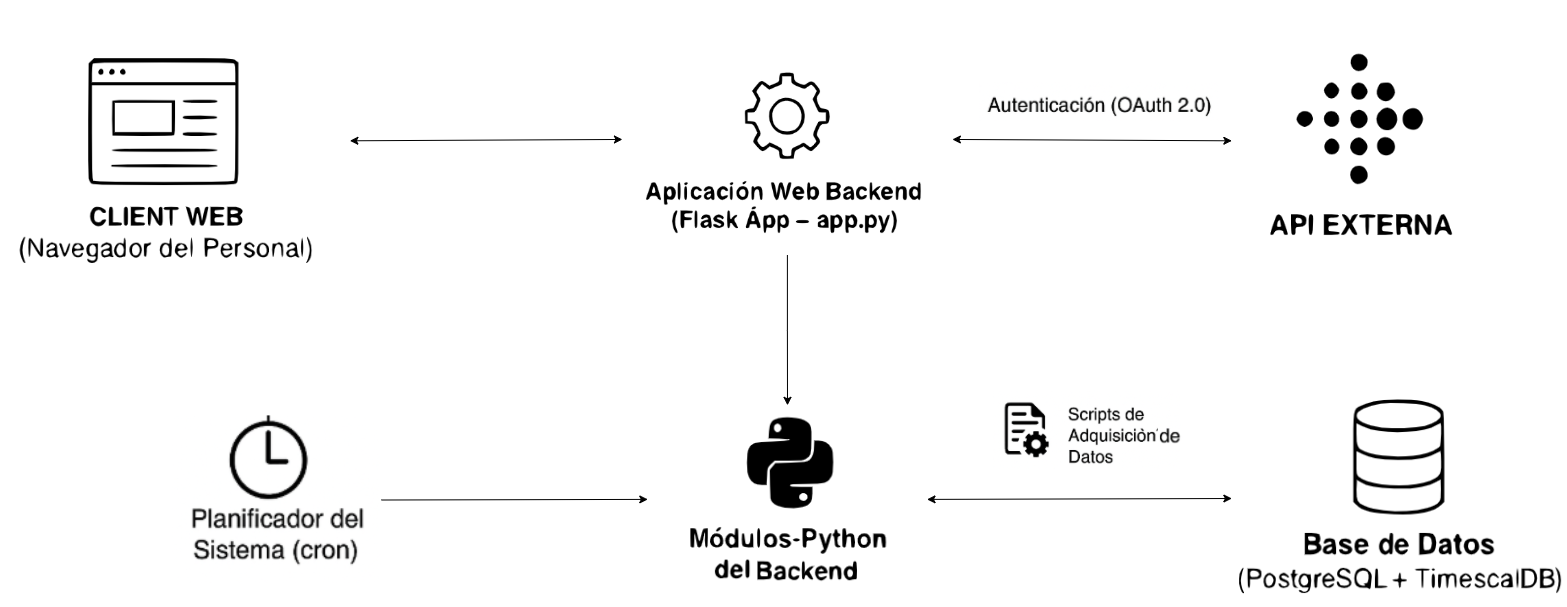
\includegraphics[width=0.9\textwidth]{imagenes/arquitectura_general.png}
    \caption{Arquitectura General del Sistema de Monitorización.}
    \label{fig:arquitectura_general}
 \end{figure}

\textit{(Descripción conceptual de la Figura \ref{fig:arquitectura_general}):}
\begin{itemize}
    \item \textbf{Cliente Web (Navegador del Personal):} Interfaz de usuario HTML/CSS/JavaScript renderizada por Flask, con plantillas Jinja2 y visualizaciones interactivas implementadas con Chart.js. El sistema está diseñado desde el backend para soportar internacionalización (español/inglés), mejorando la accesibilidad y usabilidad para diferentes perfiles de usuario.
    \item \textbf{Aplicación Web Backend (Flask App - \texttt{app.py}):} Punto de entrada principal para las interacciones del personal. Gestiona autenticación, interfaz/lógica de vinculación, y sirve las páginas del dashboard y APIs internas. La arquitectura desacopla la lógica de negocio (gestión de usuarios, tokens, alertas) de la presentación, facilitando la escalabilidad y el mantenimiento.
    \item \textbf{Módulos Python del Backend:} Componentes lógicos como \texttt{auth.py}, \texttt{db.py}, \texttt{encryption.py} utilizados por la app Flask y los scripts.
    \item \textbf{Scripts de Adquisición de Datos (\texttt{fitbit.py}, \texttt{fitbit\_intraday.py}):} Procesos Python independientes para obtener datos diarios e intradía de la API Fitbit, manejando tokens y almacenamiento. Esta separación permite que la adquisición de datos no bloquee la aplicación web y pueda escalarse o adaptarse a nuevas fuentes de datos en el futuro.
    \item \textbf{Planificador del Sistema (`cron`):} Utilidad del sistema operativo que ejecuta periódicamente los scripts de adquisición (\texttt{.sh}).
    \item \textbf{Base de Datos (PostgreSQL + TimescaleDB):} Instancia PostgreSQL con tabla relacional \texttt{users} (configuración, tokens cifrados) y hipertables TimescaleDB para datos de series temporales.
    \item \textbf{API Externa de Fitbit\textsuperscript{\textregistered}:} Servicio externo que provee los datos y maneja la autorización OAuth 2.0.
\end{itemize}   
La arquitectura está diseñada para minimizar la exposición de datos sensibles: los tokens de acceso y refresco se almacenan cifrados y nunca se exponen en el frontend, y todas las operaciones críticas se realizan en el backend autenticado. Esta estructura modular y segura facilita la mantenibilidad, la escalabilidad y el cumplimiento de los requisitos de privacidad.

\section{Diseño del Backend (Aplicación Flask y Scripts)}
\label{sec:diseno_backend}

El backend se compone de dos partes principales que interactúan a través de la base de datos:

\begin{enumerate}
    \item \textbf{Aplicación Web Flask (\texttt{app.py}):} Actúa como el servidor web principal y gestiona las interacciones síncronas del personal. Utiliza Flask-Login para la autenticación (compartida) y protege todas las rutas críticas, asegurando que solo usuarios autenticados puedan acceder a los datos sensibles. El sistema soporta internacionalización mediante Flask-Babel y plantillas multilenguaje, permitiendo cambiar el idioma de la interfaz de forma dinámica. La lógica de negocio está modularizada en diferentes archivos (\texttt{auth.py}, \texttt{db.py}, etc.), facilitando el mantenimiento y la extensión del sistema. El backend implementa una API REST interna para operaciones AJAX (precarga de dashboard, exportación de datos, actualización dinámica de alertas), mejorando la experiencia de usuario y la eficiencia. Además, se ha diseñado un sistema de logs y manejo robusto de errores para registrar incidencias y facilitar el diagnóstico. Entre sus responsabilidades clave destacan:
        \begin{itemize}
            \item Servir las páginas HTML para el login, la selección de email, la asignación de nombre y las confirmaciones (usando plantillas Jinja2 multilenguaje).
            \item Gestionar el flujo OAuth 2.0: generar parámetros (`state`, `code\_challenge`), construir la URL de autorización, manejar la redirección del usuario a Fitbit\textsuperscript{\textregistered} y procesar el `callback`.
            \item Interactuar con \texttt{auth.py} para obtener los tokens a partir del código de autorización.
            \item Interactuar con \texttt{db.py} y \texttt{encryption.py} para guardar/actualizar la información del usuario y los tokens cifrados en la tabla \texttt{users}.
            \item Servir el dashboard y exponer endpoints API para la precarga y actualización eficiente de datos, optimizando la latencia y la escalabilidad.
            \item Gestionar logs y errores de forma centralizada para garantizar la robustez del sistema.
        \end{itemize}

    \item \textbf{Scripts de Adquisición de Datos (\texttt{fitbit.py}, \texttt{fitbit\_intraday.py}):} Son procesos Python independientes ejecutados por `cron`. Cada script típicamente realiza un bucle sobre los usuarios activos recuperados de la base de datos (\texttt{db.py}) y para cada uno:
        \begin{itemize}
            \item Obtiene y descifra los tokens (\texttt{encryption.py}, \texttt{db.py}).
            \item Verifica la validez del token de acceso (\texttt{expires\_at}). Si es necesario, intenta refrescarlo usando el token de refresco (\texttt{auth.py}, \texttt{fitbit.py}) y actualiza los tokens cifrados y la expiración en la BD (\texttt{db.py}).
            \item Si los tokens son válidos, realiza las llamadas correspondientes a la API de Fitbit\textsuperscript{\textregistered} (\texttt{fitbit.py}, \texttt{fitbit\_intraday.py}).
            \item Procesa la respuesta JSON y maneja posibles errores, registrando los fallos y continuando con el siguiente usuario para garantizar la robustez.
            \item Se conecta a la BD (\texttt{db.py}) para insertar los datos procesados en las tablas/hipertablas de TimescaleDB apropiadas.
            \item Tras la inserción, ejecuta la lógica de evaluación de alertas de forma desacoplada, permitiendo la extensión futura a reglas más complejas o nuevos tipos de datos.
        \end{itemize}
\end{enumerate}
Esta separación y modularidad permiten que la adquisición de datos no bloquee la aplicación web, facilitan la escalabilidad (añadiendo más scripts o fuentes de datos) y mejoran la mantenibilidad del sistema.

\section{Diseño de la Base de Datos (PostgreSQL + TimescaleDB)}
\label{sec:diseno_bd}

Se utiliza una única base de datos \textbf{PostgreSQL}, aprovechando la extensión \textbf{TimescaleDB} para optimizar el manejo de datos de series temporales. La elección de TimescaleDB se debe a su integración nativa con PostgreSQL, su soporte para consultas SQL estándar y su capacidad para gestionar grandes volúmenes de datos temporales de forma eficiente, lo que resulta especialmente adecuado para aplicaciones de monitorización continua.

El diseño se basa en una tabla relacional para la gestión de usuarios y vinculaciones, y un conjunto de hipertables para los datos temporales. La normalización del modelo permite mantener la integridad y facilitar la extensión futura (por ejemplo, añadiendo nuevas métricas o tipos de alertas).

\begin{itemize}
    \item \textbf{Tabla \texttt{users}:} Almacena la información básica de los usuarios y la vinculación con Fitbit\textsuperscript{\textregistered}, incluyendo nombre, email y credenciales cifradas. Es la tabla central para la gestión de usuarios y la referencia de integridad en el resto del modelo.
    \item \textbf{Hipertabla \texttt{daily\_summaries}:} Guarda los resúmenes diarios de actividad, sueño y biomarcadores para cada usuario y fecha. Permite analizar tendencias y detectar cambios relevantes en la salud.
    \item \textbf{Hipertabla \texttt{intraday\_metrics}:} Registra datos de alta frecuencia (minuto a minuto u hora a hora) como pasos, frecuencia cardíaca, calorías, etc. Es clave para la detección de patrones y anomalías intradía.
    \item \textbf{Hipertabla \texttt{sleep\_logs}:} Almacena episodios de sueño detallados, incluyendo fases y eficiencia, para cada usuario. Permite análisis avanzados de calidad y patrones de sueño.
    \item \textbf{Hipertabla \texttt{alerts}:} Registra todas las alertas generadas por el sistema, asociando cada evento con el usuario, el tipo de alerta, prioridad, valores disparadores y detalles. Es la base para la visualización y gestión clínica de incidencias.
\end{itemize}

La Figura~\ref{fig:esquema_relacional} muestra el esquema relacional completo, incluyendo las claves primarias y foráneas que aseguran la integridad referencial entre las tablas.

\begin{figure}[htbp]
    \centering
    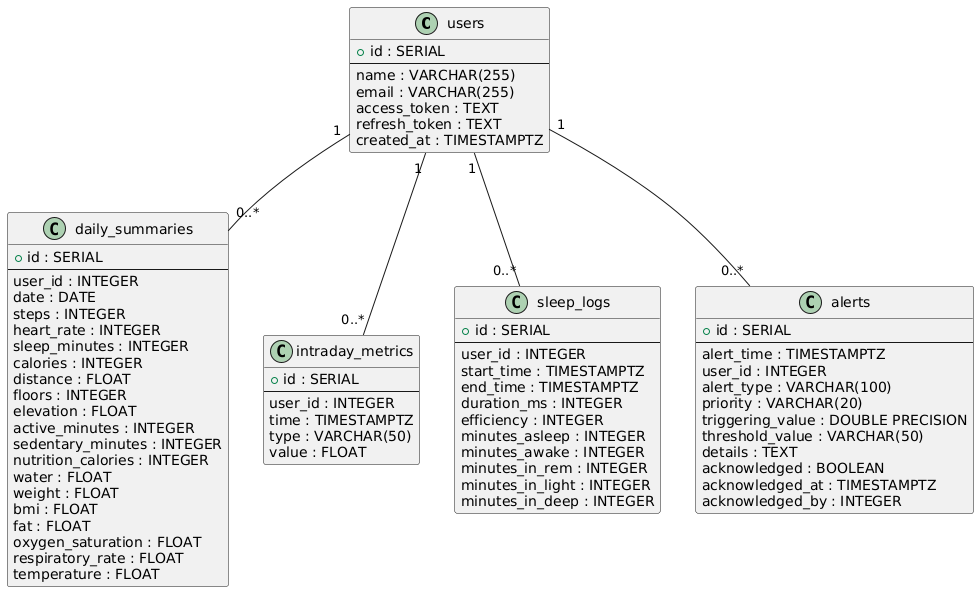
\includegraphics[width=0.9\textwidth]{imagenes/esquema_relacional.png}
    \caption{Esquema relacional de la base de datos del sistema.}
    \label{fig:esquema_relacional}
\end{figure}

El detalle de las sentencias SQL \texttt{CREATE TABLE} y la explicación de cada campo se encuentra en el \textbf{Anexo~\ref{app:db_schema}}.

\section{Diseño de la Integración con Fitbit}
\label{sec:diseno_integracion_fitbit}

La integración con la API de Fitbit\textsuperscript{\textregistered} se ha diseñado priorizando la seguridad, la robustez y el cumplimiento normativo (RGPD). El sistema utiliza el flujo OAuth 2.0 con PKCE, estándar para aplicaciones web, que protege frente a ataques de interceptación y CSRF. La lógica de autenticación y autorización está desacoplada de la adquisición y almacenamiento de datos, permitiendo una gestión segura y flexible de los tokens.

Los tokens de acceso y refresco se cifran inmediatamente tras su obtención y se almacenan en la base de datos, utilizando una clave secreta gestionada como variable de entorno (nunca en el código fuente). Los tokens solo se descifran en memoria cuando es necesario realizar una llamada a la API o refrescarlos.

El sistema implementa una gestión robusta de tokens: antes de cada acceso a datos protegidos, se verifica la validez del token de acceso y, si es necesario, se utiliza el token de refresco para obtener uno nuevo. Si el refresco falla (por ejemplo, si el usuario ha revocado permisos), se notifica la incidencia y se requiere reautorizar la vinculación.

La arquitectura modular permite, en el futuro, integrar otras APIs de dispositivos o servicios de salud con mínimos cambios en la lógica de autenticación y almacenamiento seguro.

\begin{itemize}
    \item \textbf{OAuth 2.0 con PKCE:} Se implementa el flujo Authorization Code Grant con PKCE para la vinculación inicial, utilizando parámetros de seguridad como \texttt{state} y \texttt{code\_challenge}.
    \item \textbf{Gestión segura de tokens:} Los tokens se cifran antes de almacenarse y solo se descifran en memoria cuando es imprescindible. La clave de cifrado se gestiona externamente.
    \item \textbf{Refresco automático y robusto:} El sistema refresca los tokens de forma transparente y registra cualquier error o revocación, permitiendo la intervención manual si es necesario.
    \item \textbf{Control de errores y versionado:} Se gestionan los códigos de estado HTTP y el versionado de la API, asegurando la compatibilidad y la robustez ante cambios o incidencias externas.
\end{itemize}

\section{Diseño del Pipeline de Datos}
\label{sec:diseno_pipeline}

El pipeline de datos del sistema está diseñado para garantizar la adquisición, validación, almacenamiento y análisis eficiente de la información proveniente de los dispositivos Fitbit, así como su posterior visualización y explotación clínica. El flujo general es el siguiente:

\begin{enumerate}
    \item \textbf{Orquestación por cron:} El planificador del sistema operativo (\texttt{cron}) ejecuta periódicamente los scripts de adquisición (\texttt{fitbit.py}, \texttt{fitbit\_intraday.py}) mediante scripts \texttt{.sh}.
    \item \textbf{Adquisición y validación:} Cada script obtiene la lista de usuarios y sus credenciales cifradas desde la base de datos, descifra los tokens y valida/refresca el acceso a la API de Fitbit. Si hay errores de autenticación, se registran y se continúa con el siguiente usuario.
    \item \textbf{Obtención y almacenamiento de datos:} Para cada usuario, se descargan los datos diarios e intradía, se validan y se insertan en las hipertablas correspondientes de TimescaleDB (\texttt{daily\_summaries}, \texttt{intraday\_metrics}, \texttt{sleep\_logs}).
    \item \textbf{Evaluación de alertas:} Tras la inserción de nuevos datos, se ejecuta la lógica de evaluación de alertas (módulo \texttt{alert\_rules.py}), que compara los datos recientes con los umbrales definidos y registra cualquier evento relevante en la tabla \texttt{alerts}.
    \item \textbf{Visualización y explotación:} El backend Flask expone endpoints y plantillas que permiten al personal consultar, filtrar y exportar los datos y alertas, incluyendo la precarga eficiente del dashboard y la optimización de consultas para mejorar la experiencia de usuario.
\end{enumerate}

Este diseño desacopla completamente la adquisición y análisis de datos de la visualización, permitiendo escalar ambos componentes de forma independiente y facilitando la integración futura de nuevas fuentes de datos o reglas de alerta.

\vspace{0.5cm}

El flujo de datos, desde la adquisición en la API de Fitbit hasta la visualización en el dashboard, se resume en la Figura~\ref{fig:flujo_datos}. Este diagrama ilustra los pasos principales: adquisición, almacenamiento, procesamiento de alertas y visualización.

\begin{figure}[htbp]
    \centering
    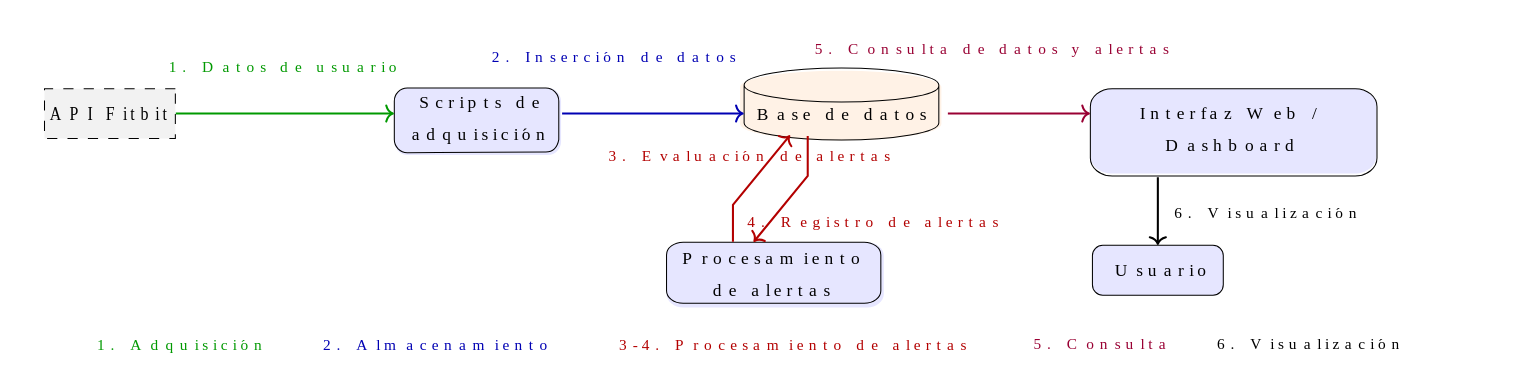
\includegraphics[width=1\textwidth, height=0.3\textheight]{imagenes/flujo_datos.png}
    \caption{Flujo de datos desde la API de Fitbit hasta la visualización en el dashboard.}
    \label{fig:flujo_datos}
\end{figure}

\subsection{Evaluación Dinámica de Reglas de Alerta}
La detección de anomalías y generación de alertas se realiza de forma automática tras cada ingesta de datos, mediante funciones desacopladas del frontend y definidas en un módulo específico. Las reglas pueden consultar ventanas temporales (por ejemplo, 7 días de pasos o sueño) y comparar los valores actuales con medias, umbrales o desviaciones estándar. El resultado se almacena en la tabla \texttt{alerts}, permitiendo su posterior revisión clínica.

El diseño modular facilita la incorporación de nuevas reglas, la extensión a patrones más complejos o incluso la integración futura de algoritmos de aprendizaje automático.

\section{Diseño de la Interfaz de Usuario}
\label{sec:diseno_ui}

La interfaz de usuario (UI) del sistema está diseñada para ser intuitiva, accesible y eficiente, facilitando tanto la gestión administrativa como la visualización clínica de los datos monitorizados. Se compone de dos grandes bloques:

\begin{itemize}
    \item \textbf{Interfaz de Gestión y Vinculación (Flask/HTML + Bootstrap):}
        \begin{itemize}
            \item Implementada mediante plantillas Jinja2 renderizadas por Flask (\texttt{app.py}), con soporte completo para internacionalización (español/inglés).
            \item Incluye páginas para login, vinculación de dispositivos, asignación y reasignación de usuarios, y confirmaciones de acciones.
            \item Utiliza formularios HTML y Bootstrap para garantizar una experiencia de usuario moderna y responsiva.
            \item El flujo de vinculación guía al usuario de forma clara a través del proceso OAuth 2.0, mostrando mensajes de error y confirmación según corresponda.
        \end{itemize}
    \item \textbf{Dashboard de Visualización y Alertas:}
        \begin{itemize}
            \item Implementado como un conjunto de vistas Flask con plantillas Jinja2 y componentes interactivos (JavaScript, Chart.js).
            \item Permite visualizar resúmenes diarios, métricas intradía, patrones de sueño y alertas recientes para cada usuario.
            \item Incluye filtros avanzados (por usuario, fecha, tipo de alerta, prioridad, etc.) y opciones de exportación a CSV.
            \item La precarga de datos y la optimización de consultas mejoran la velocidad de carga y la experiencia de usuario, especialmente en el dashboard de alertas.
            \item El diseño es accesible y responsivo, adaptándose a diferentes dispositivos y perfiles de usuario.
        \end{itemize}
\end{itemize}

La interfaz está pensada para facilitar la labor clínica y administrativa, permitiendo identificar rápidamente incidencias relevantes y acceder a los datos históricos de cada usuario. La modularidad y el uso de tecnologías estándar (Flask, Bootstrap, Chart.js) aseguran la mantenibilidad y la posibilidad de futuras ampliaciones.

\subsection*{Ficha de Usuario y Visualización Individual}
Una de las vistas más relevantes del sistema es la \textbf{ficha de usuario} (\texttt{user\_detail.html}), que centraliza toda la información relevante de cada paciente o usuario monitorizado. Esta vista está diseñada para facilitar la toma de decisiones clínicas y el seguimiento personalizado, integrando:

\begin{itemize}
    \item \textbf{Resumen de datos personales:} nombre, email, fecha de registro y estado de actividad reciente.
    \item \textbf{Métricas clave del día:} pasos, frecuencia cardíaca, horas de sueño, calorías, etc., resaltando visualmente cualquier valor anómalo o alerta activa.
    \item \textbf{Alertas recientes:} listado de alertas generadas en los últimos días, con posibilidad de reconocerlas directamente desde la ficha.
    \item \textbf{Gráficos interactivos:} evolución semanal de pasos, sueño, frecuencia cardíaca y minutos activos, así como visualización intradía y análisis de patrones de inactividad, implementados con Chart.js.
    \item \textbf{Tabs de navegación:} acceso rápido a diferentes vistas (resumen diario, intradía, semanal, alertas, inactividad).
    \item \textbf{Exportación y actualización:} botones para exportar datos a CSV y actualizar la información en tiempo real.
    \item \textbf{Accesibilidad y usabilidad:} diseño responsivo, iconografía clara, leyendas de colores para priorización y mensajes de estado.
\end{itemize}

Esta ficha ejemplifica la integración de todos los módulos del sistema (adquisición, almacenamiento, análisis y visualización), permitiendo al personal sanitario o gestor acceder de forma rápida y comprensible a la información más relevante para cada usuario.

\subsection{Diseño del Módulo de Alertas}
\label{subsec:diseno_alertas}

El módulo de alertas es un componente central del sistema, encargado de analizar los datos almacenados y detectar automáticamente situaciones clínicas relevantes o anomalías en la actividad, el sueño o la frecuencia cardíaca de los usuarios. Su diseño es modular y desacoplado del frontend, permitiendo su ejecución periódica tras cada ingesta de datos y facilitando la extensión futura con nuevas reglas o métricas.

\begin{itemize}
    \item \textbf{Acceso a datos históricos:} El módulo dispone de funciones específicas (en \texttt{db.py}) para recuperar las métricas necesarias en ventanas temporales (por ejemplo, los últimos 7 días de pasos o sueño) y realizar comparaciones con la línea base individual de cada usuario.
    \item \textbf{Lógica de comparación y reglas:} Las reglas de alerta están implementadas en Python (\texttt{alert\_rules.py}) y se basan en umbrales científicos, porcentajes de cambio, desviaciones estándar o rangos fisiológicos. Cada función evalúa si los datos actuales superan los límites definidos y, en caso afirmativo, genera una alerta con prioridad, tipo, valor disparador y detalles clínicos.
    \item \textbf{Registro y gestión de alertas:} Las alertas detectadas se almacenan en la tabla \texttt{alerts}, asociando cada evento con el usuario, la métrica, la prioridad y una descripción. Esto permite su posterior visualización, filtrado y exportación desde el dashboard.
    \item \textbf{Extensibilidad:} El diseño permite añadir fácilmente nuevas reglas, métricas o fuentes de datos, así como adaptar los umbrales según la evidencia clínica o la experiencia práctica.
\end{itemize}

\subsubsection*{Manejo de Datos Faltantes o Erróneos}
La calidad de los datos de wearables puede verse afectada por desconexiones, falta de uso o errores de medición. El sistema implementa estrategias robustas para minimizar falsas alarmas y garantizar la fiabilidad de las alertas:
\begin{itemize}
    \item Se requiere un porcentaje mínimo de días con datos válidos en las ventanas temporales para evaluar una alerta (por ejemplo, al menos 5 de 7 días).
    \item Se aplican filtros de rango fisiológico antes de procesar los datos (por ejemplo, descartar valores de frecuencia cardíaca fuera de 30-200 bpm o pasos diarios superiores a 50.000).
    \item Los datos faltantes críticos generan alertas de calidad de datos, permitiendo al personal identificar posibles problemas de uso o sincronización.
\end{itemize}

\subsubsection*{Optimización y Rendimiento}
Dado el volumen potencial de datos y la necesidad de evaluaciones históricas frecuentes, el sistema optimiza el acceso y procesamiento mediante:
\begin{itemize}
    \item Índices compuestos en las hipertablas de TimescaleDB (por ejemplo, sobre \texttt{(user\_id, time)}) para acelerar las consultas.
    \item Cálculos eficientes en los scripts, reutilizando los datos recuperados para varias métricas cuando es posible.
    \item Procesamiento asíncrono y desacoplado mediante la ejecución periódica por \texttt{cron}, evitando que la evaluación de alertas afecte la experiencia de usuario en la interfaz web.
\end{itemize}

\subsubsection*{Diagrama de Flujo del Proceso de Detección de Alertas}
El proceso lógico para la detección y registro de alertas sigue el flujo ilustrado en la Figura~\ref{fig:diagrama_alertas}:

\begin{figure}[htbp]
    \centering
    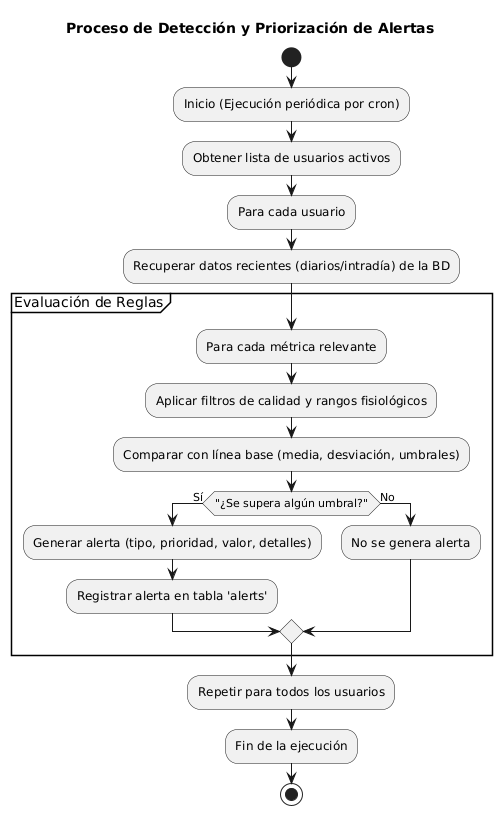
\includegraphics[width=0.9\textwidth,height=0.6\textheight]{imagenes/diagrama_alertas.png} 
    \caption{Diagrama de flujo del proceso de detección y priorización de alertas. Muestra la obtención de datos, preprocesamiento, evaluación de criterios individuales y combinados, asignación de prioridad y registro.}
    \label{fig:diagrama_alertas}
\end{figure}

Este diseño permite que la evaluación de alertas se beneficie de las optimizaciones de consulta de TimescaleDB y se mantenga desacoplada de la interfaz de usuario, garantizando robustez, escalabilidad y relevancia clínica.

\subsection{Arquitectura de la Interfaz Web y Dashboards}
\label{sec:arquitectura_dashboard}

La interfaz web del sistema está compuesta por dos dashboards principales:

\begin{itemize}
    \item \textbf{Dashboard de Alertas:} Permite al personal autorizado visualizar, filtrar y exportar todas las alertas generadas por el sistema. Incluye filtros por fecha, usuario, tipo de alerta, prioridad y estado de reconocimiento. Cada alerta puede ser reconocida manualmente y se muestra información detallada, incluyendo datos intradía relevantes y contexto clínico.
    \item \textbf{Dashboard de Usuarios:} Presenta un listado de todos los usuarios monitorizados, con búsqueda por nombre o email y estado de actividad reciente. Desde aquí se accede a la ficha de usuario.
\end{itemize}

La \textbf{ficha de usuario} incluye:
\begin{itemize}
    \item Resumen diario de métricas clave (pasos, frecuencia cardíaca, sueño, calorías, etc.).
    \item Visualización de datos intradía (gráficos de pasos, FC, calorías, minutos activos).
    \item Resumen semanal (tendencias de pasos, sueño, actividad, etc.).
    \item Listado de alertas recientes y posibilidad de exportarlas.
    \item Análisis de patrones de inactividad (detección de periodos prolongados sin actividad).
    \item Exportación de datos históricos e intradía en formato CSV.
\end{itemize}

La navegación entre dashboards y fichas de usuario es intuitiva y está protegida por autenticación. El diseño prioriza la claridad visual y la accesibilidad para facilitar la toma de decisiones clínicas.

\input{capitulos/5implementación.tex}
\input{capitulos/6pruebas_y_validación.tex}
\input{capitulos/7resultados_y_discusión.tex}
\chapter{Conclusiones y Trabajo Futuro}
% Reflexión crítica, comparación con el estado del arte


% --- Bibliografía ---
\cleardoublepage
\phantomsection
\chapter*{Bibliografía}
\addcontentsline{toc}{chapter}{Bibliografía}
\bibliographystyle{plainnat} % O el estilo que necesites
\bibliography{referencias.bib} % Tu archivo .bib
% --- Anexos ---
\cleardoublepage
\appendix % ¡Importante! Indica que empiezan los anexos (A, B, C...)
\begin{appendices} % Alternativa si tienes varios capítulos de anexos

% -*- coding: utf-8 -*-
% Contenido del Anexo A

% Añadir al índice manualmente y asegurar anclaje correcto para hyperref
\chapter{Esquema Detallado de la Base de Datos} 
\label{app:db_schema} % Etiqueta para referenciar con \ref{}

Este anexo contiene las definiciones SQL (\texttt{CREATE TABLE}) detalladas para todas las tablas principales del sistema, incluyendo la tabla relacional \texttt{users} y las hipertablas para datos de series temporales y alertas. Se recomienda consultar la Figura~\ref{fig:esquema_relacional} para una visión global de las relaciones.

% Esquema relacional generado a partir del modelo real (ver PlantUML adjunto)
\begin{figure}[htbp]
    \centering
    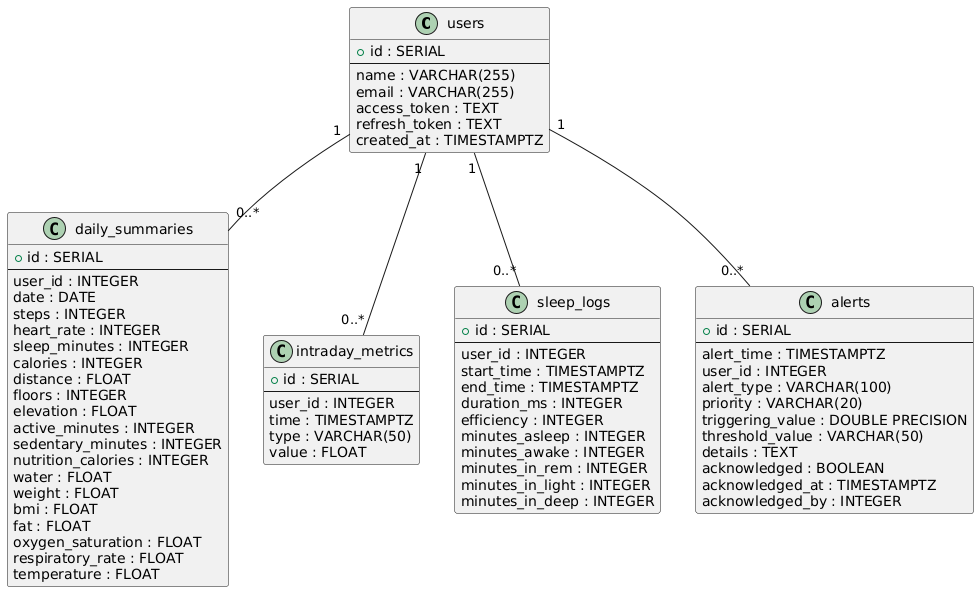
\includegraphics[width=0.9\textwidth]{imagenes/esquema_relacional.png}
    \caption{Esquema relacional de la base de datos del sistema.}
    \label{fig:esquema_relacional}
\end{figure}

\section*{Descripción de las tablas principales}
\begin{itemize}
    \item \textbf{users}: Información básica y credenciales cifradas de los usuarios.
    \item \textbf{daily\_summaries}: Resúmenes diarios de actividad, sueño y biomarcadores.
    \item \textbf{intraday\_metrics}: Datos de alta frecuencia (pasos, FC, calorías, etc.).
    \item \textbf{sleep\_logs}: Episodios de sueño detallados.
    \item \textbf{alerts}: Alertas generadas por el sistema, asociadas a usuario y condición detectada.
\end{itemize}

\section*{Tabla \texttt{users}}
Tabla relacional estándar para almacenar la información de vinculación de usuarios y credenciales cifradas.

\begin{verbatim}
CREATE TABLE IF NOT EXISTS users (
    id SERIAL PRIMARY KEY,
    name VARCHAR(255) NOT NULL,
    email VARCHAR(255) NOT NULL,
    access_token TEXT,
    refresh_token TEXT,
    created_at TIMESTAMPTZ DEFAULT CURRENT_TIMESTAMP
);
\end{verbatim}

\section*{Hipertabla \texttt{intraday\_metrics}}
Almacena datos intradía (pasos, frecuencia cardíaca, calorías, etc.) con referencia al usuario.

\begin{verbatim}
CREATE TABLE IF NOT EXISTS intraday_metrics (
    id SERIAL PRIMARY KEY,
    user_id INTEGER REFERENCES users(id),
    time TIMESTAMPTZ NOT NULL,
    type VARCHAR(50) NOT NULL,
    value FLOAT NOT NULL
);
SELECT create_hypertable('intraday_metrics', 'time', if_not_exists => TRUE, migrate_data => TRUE);
\end{verbatim}

\section*{Hipertabla \texttt{daily\_summaries}}
Almacena resúmenes diarios de actividad, sueño y biomarcadores.

\begin{verbatim}
CREATE TABLE IF NOT EXISTS daily_summaries (
    id SERIAL PRIMARY KEY,
    user_id INTEGER REFERENCES users(id),
    date DATE NOT NULL,
    steps INTEGER,
    heart_rate INTEGER,
    sleep_minutes INTEGER,
    calories INTEGER,
    distance FLOAT,
    floors INTEGER,
    elevation FLOAT,
    active_minutes INTEGER,
    sedentary_minutes INTEGER,
    nutrition_calories INTEGER,
    water FLOAT,
    weight FLOAT,
    bmi FLOAT,
    fat FLOAT,
    oxygen_saturation FLOAT,
    respiratory_rate FLOAT,
    temperature FLOAT,
    UNIQUE(user_id, date)
);
SELECT create_hypertable('daily_summaries', 'date', if_not_exists => TRUE, migrate_data => TRUE);
\end{verbatim}

\section*{Hipertabla \texttt{sleep\_logs}}
Registra episodios de sueño detallados por usuario.

\begin{verbatim}
CREATE TABLE IF NOT EXISTS sleep_logs (
    id SERIAL PRIMARY KEY,
    user_id INTEGER REFERENCES users(id),
    start_time TIMESTAMPTZ NOT NULL,
    end_time TIMESTAMPTZ NOT NULL,
    duration_ms INTEGER,
    efficiency INTEGER,
    minutes_asleep INTEGER,
    minutes_awake INTEGER,
    minutes_in_rem INTEGER,
    minutes_in_light INTEGER,
    minutes_in_deep INTEGER
);
SELECT create_hypertable('sleep_logs', 'start_time', if_not_exists => TRUE, migrate_data => TRUE);
\end{verbatim}

\section*{Hipertabla \texttt{alerts}}
Almacena las alertas generadas por el sistema, referenciando al usuario y con detalles de la condición detectada.

\begin{verbatim}
CREATE TABLE IF NOT EXISTS alerts (
    id SERIAL PRIMARY KEY,
    alert_time TIMESTAMPTZ DEFAULT CURRENT_TIMESTAMP,
    user_id INTEGER REFERENCES users(id),
    alert_type VARCHAR(100) NOT NULL,
    priority VARCHAR(20) NOT NULL,
    triggering_value DOUBLE PRECISION,
    threshold_value VARCHAR(50),
    details TEXT,
    acknowledged BOOLEAN DEFAULT FALSE
);
SELECT create_hypertable('alerts', 'alert_time', if_not_exists => TRUE, migrate_data => TRUE);
\end{verbatim} 

\chapter{Validación y Ajuste del Sistema de Alertas}
\label{anexo:validacion_alertas}

% !TEX root = ../main.tex % Indica a algunos editores cuál es el fichero raíz
\chapter{Anexos de Código de Implementación Especifico} % Título consistente con Anexo A
\label{anexo:implementacion_detalles} % Etiqueta general para el anexo

% --- Sección de crontab ---
\section{Configuración de \texttt{cron}}
\label{annex:code:crontab}
Ejemplo de la configuración utilizada en \texttt{crontab} para la ejecución periódica de los scripts de adquisición de datos, asegurando que se ejecuten dentro del entorno virtual correcto y redirigiendo la salida a ficheros de log.
\begin{lstlisting}[language=bash, caption={Ejemplo de configuración de crontab para scripts de adquisición.}, label={lst:crontab_example}]
# Activar entorno virtual y ejecutar script de datos diarios dos veces al dia
# Ejecutar a las 9:05 y 22:05 cada día
5 9,22 * * * cd /ruta/completa/al/proyecto && /ruta/completa/al/venv/bin/python fitbit.py >> /ruta/completa/al/proyecto/logs/cron_daily.log 2>&1

# Activar entorno virtual y ejecutar script de datos intradia cada 15 minutos
# Ejecutar en los minutos 0, 15, 30, 45 de cada hora
*/15 * * * * cd /ruta/completa/al/proyecto && /ruta/completa/al/venv/bin/python fitbit_intraday.py >> /ruta/completa/al/proyecto/logs/cron_intraday.log 2>&1
\end{lstlisting}
\textit{Nota: Las rutas (\texttt{/ruta/completa/al/...}) deben reemplazarse por las rutas absolutas correctas en el sistema de despliegue.}

% --- Sección de inserción ---
\section{Función de Inserción en TimescaleDB (\texttt{insert\_intraday\_metrics})}
\label{annex:code:insert_intraday}
Ejemplo de función en \texttt{db.py} para insertar eficientemente datos en la hipertabla \texttt{intraday\_metrics} utilizando \texttt{psycopg2.extras.execute\_values}. Incluye manejo básico de errores y conflictos.
\begin{lstlisting}[caption={Ejemplo de función de inserción masiva en TimescaleDB (\texttt{db.py}).}, label={lst:insert_intraday_code}]
import psycopg2
from psycopg2.extras import execute_values # Para inserción eficiente
import logging # Mejor usar logging que print para mensajes

# Configurar logging (preferiblemente al inicio de db.py o app.py)
logging.basicConfig(level=logging.INFO, format='%(asctime)s - %(levelname)s - %(message)s')

# Asumiendo que 'conn' es una conexión psycopg2 válida

def insert_intraday_metrics(conn, data_list):
    """
    Inserta una lista de métricas intradía en la hipertabla.
    data_list: lista de tuplas [(time, user_email, type, value), ...]
                time debe ser un objeto datetime con timezone (idealmente UTC).
    """
    if not data_list:
        logging.info("No hay datos intradía para insertar.")
        return True # Nada que insertar

    sql = """
        INSERT INTO intraday_metrics (time, user_email, type, value)
        VALUES %s
        ON CONFLICT (time, user_email, type) DO NOTHING;
        -- Estrategia de conflicto: Ignorar duplicados.
        -- Alternativa: ON CONFLICT (time, user_email, type)
        -- DO UPDATE SET value = EXCLUDED.value; (Actualizar si existe)
    """
    cursor = None # Inicializar cursor fuera del try para el finally
    try:
        cursor = conn.cursor()
        # execute_values es eficiente para inserciones múltiples
        execute_values(cursor, sql, data_list, page_size=100) # page_size ajustable
        conn.commit()
        logging.info(f"Insertadas/Ignoradas {len(data_list)} métricas intradía.")
        return True
    except (Exception, psycopg2.DatabaseError) as error:
        logging.error(f"Error insertando métricas intradía: {error}")
        if conn:
            conn.rollback() # Deshacer transacción en caso de error
        return False
    finally:
        if cursor:
            cursor.close() # Siempre cerrar el cursor

# --- Ejemplo de preparación de datos en fitbit_intraday.py ---
# (Incluir ejemplo de parsing de tiempo y construcción de data_list
#  como en la respuesta anterior, asegurando manejo de timezone)
# from datetime import datetime, timezone
# import pytz
# ... (código de parse_fitbit_time y bucle de procesamiento) ...
\end{lstlisting}
\textit{Nota: La implementación real debe incluir un manejo robusto de zonas horarias, errores de parsing y podría beneficiarse de logging más detallado.}

% --- Sección de consulta ---
\section{Función de Consulta en TimescaleDB (\texttt{get\_hr\_data})}
\label{annex:code:get_hr}
Ejemplo esquemático de una función en \texttt{db.py} para recuperar datos de frecuencia cardíaca para el dashboard, filtrando por usuario y rango de tiempo.
\begin{lstlisting}[caption={Ejemplo de función de consulta de FC (\texttt{db.py}).}, label={lst:get_hr_code}]
import psycopg2
from datetime import datetime
import logging
# import pandas as pd # Opcional: devolver como DataFrame

def get_hr_data(conn, user_email: str, start_date: datetime, end_date: datetime):
    """
    Recupera datos de frecuencia cardíaca para un usuario en un rango de fechas.
    start_date y end_date deben ser objetos datetime (preferiblemente aware, UTC).
    """
    # Asegurarse que las fechas de entrada son conscientes de zona horaria si es necesario
    # O convertir a UTC si la columna 'time' está en UTC
    # Ejemplo: Asumiendo que start/end_date son naive, y BD está en UTC
    # start_date_utc = start_date.replace(tzinfo=timezone.utc)
    # end_date_utc = end_date.replace(tzinfo=timezone.utc)

    sql = """
        SELECT time, value
        FROM intraday_metrics
        WHERE user_email = %s
          AND type = 'heart_rate'
          AND time >= %s -- Fecha/hora de inicio inclusiva
          AND time < %s  -- Fecha/hora de fin exclusiva
        ORDER BY time ASC;
    """
    results = []
    cursor = None
    try:
        cursor = conn.cursor()
        # Pasar las fechas como parámetros
        cursor.execute(sql, (user_email, start_date, end_date))
        results = cursor.fetchall() # Lista de tuplas [(time, value), ...]
        logging.info(f"Recuperados {len(results)} puntos de FC para {user_email}.")

        # --- Opcional: Convertir a DataFrame de Pandas ---
        # if results:
        #     df = pd.DataFrame(results, columns=['time', 'value'])
        #     # Asegurar que la columna de tiempo sea datetime y tenga timezone
        #     df['time'] = pd.to_datetime(df['time'], utc=True)
        #     return df
        # else:
        #     # Devolver DataFrame vacío con columnas definidas
        #     return pd.DataFrame(columns=['time', 'value'])
        # --- Fin Opcional Pandas ---

        return results # Devuelve lista de tuplas por defecto
    except (Exception, psycopg2.DatabaseError) as error:
        logging.error(f"Error recuperando datos de FC para {user_email}: {error}")
        # return pd.DataFrame(columns=['time', 'value']) # O DataFrame vacío
        return [] # Lista vacía en caso de error
    finally:
        if cursor:
            cursor.close()

# --- Ejemplo de uso en el callback del dashboard ---
# db_conn = db.connect_to_db()
# if db_conn:
#     hr_data_tuples = db.get_hr_data(db_conn, selected_email, start_dt_obj, end_dt_obj)
#     db_conn.close()
#     # Procesar hr_data_tuples para generar el gráfico Plotly...
\end{lstlisting}
\textit{Nota: El manejo preciso de las fechas y zonas horarias (\texttt{start\_date}, \texttt{end\_date}) al pasarlas a la consulta SQL es crucial y depende de cómo se almacenen en la BD (con o sin zona horaria) y cómo se reciban del DatePicker.}

% --- Sección de layout de Dash ---
\section{Layout Básico del Dashboard (\texttt{app.py} o \texttt{dashboard.py})}
\label{annex:code:dash_layout}
Estructura básica del layout de la aplicación Dash definida en Python, utilizando los componentes de \texttt{dash} para crear la interfaz interactiva.
\begin{lstlisting}[caption={Ejemplo de layout de Dash integrado en Flask.}, label={lst:dash_layout_code}]
import dash
# En versiones nuevas de Dash (>=2.0):
from dash import dcc, html
# En versiones antiguas:
# import dash_core_components as dcc
# import dash_html_components as html
from dash.dependencies import Input, Output, State
# from flask_login import login_required # Para proteger ruta Flask

# --- Asumiendo 'server' es la instancia de Flask ---
# app_dash = dash.Dash(__name__, server=server, url_base_pathname='/dashboard/')
# # Configurar Dash para servir assets locales si los tienes (CSS, JS)
# # app_dash.config.suppress_callback_exceptions = True # Si callbacks están en otro fichero

# --- Layout de Dash ---
# (Puede estar en app.py o importado de dashboard_layout.py)
# layout = html.Div([ ... ]) # Definición del layout como antes...

def create_dashboard_layout():
    """Función que devuelve el layout para permitir actualizaciones si es necesario."""
    return html.Div([
        html.H1("Panel de Monitorización de Residentes"),
        # Dropdown para seleccionar residente
        html.Div([
            html.Label("Seleccionar Residente:"),
            dcc.Dropdown(
                id='resident-dropdown',
                options=[
                    # Las opciones se cargan dinámicamente con un callback
                ],
                placeholder="Seleccione un residente...",
                clearable=False, # Evitar que quede vacío si solo hay 1 opción
                style={'width': '50%'} # Ajustar estilo si es necesario
            )
        ], style={'padding': 10}),

        # Selector de rango de fechas
        html.Div([
            html.Label("Seleccionar Rango de Fechas:"),
            dcc.DatePickerRange(
                id='date-picker-range',
                start_date_placeholder_text="Fecha Inicio",
                end_date_placeholder_text="Fecha Fin",
                display_format='YYYY-MM-DD',
                # Podrías establecer fechas iniciales por defecto
                # initial_visible_month=datetime.date.today(),
                # start_date=datetime.date.today() - datetime.timedelta(days=7),
                # end_date=datetime.date.today(),
                clearable=True,
                style={'marginLeft': '10px'}
            )
        ], style={'padding': 10, 'display': 'flex', 'alignItems': 'center'}),

        html.Hr(), # Separador visual

        # Contenedor para los gráficos (se actualizan con callbacks)
        html.Div(id='graphs-container', children=[
            html.Div([
                html.H3("Frecuencia Cardíaca"),
                dcc.Loading( # Añadir indicador de carga
                    type="default",
                    children=dcc.Graph(id='hr-graph')
                )
            ]),
            html.Div([
                html.H3("Pasos Diarios"),
                 dcc.Loading(
                    type="default",
                    children=dcc.Graph(id='steps-graph')
                 )
            ]),
            html.Div([
                html.H3("Resumen del Sueño"),
                 dcc.Loading(
                    type="default",
                    children=dcc.Graph(id='sleep-graph')
                 )
            ]),
            # Añadir más gráficos aquí si es necesario
        ])
        # dcc.Store(id='intermediate-data-store') # Para almacenar datos intermedios
    ])

# Asignar el layout a la app Dash
# app_dash.layout = create_dashboard_layout

# --- Ruta Flask para servir el dashboard ---
# @server.route('/dashboard/')
# @login_required # Proteger la ruta
# def dashboard_page():
#     # Renderizar la plantilla base de Flask que contiene el layout de Dash
#     # O directamente servir app_dash.index() si no necesitas plantilla Flask
#     return app_dash.index() # Método estándar para servir Dash standalone/integrado

\end{lstlisting}
\textit{Nota: Se han añadido componentes \texttt{dcc.Loading} para mejorar la experiencia de usuario mientras se cargan los datos.}

% --- Sección de callback de Dash ---
\section{Callback Principal del Dashboard (\texttt{app.py} o \texttt{dashboard\_callbacks.py})}
\label{annex:code:dash_callback}
Ejemplo esquemático del callback principal que actualiza los gráficos del dashboard. Muestra la estructura de inputs, outputs y la lógica de consulta y generación de figuras Plotly.
\begin{lstlisting}[caption={Ejemplo de callback principal en Dash para actualizar gráficos.}, label={lst:dash_callback_code}]
from dash.dependencies import Input, Output, State
import plotly.graph_objs as go
import plotly.express as px # Alternativa para crear figuras más rápido
from datetime import datetime, date, timedelta
import logging
# import db # Asumiendo funciones de db.py
# import pandas as pd # Si se usa Pandas para procesar

# Asumiendo 'app_dash' es la instancia de la app Dash

# --- Callback para poblar el dropdown de residentes (ejecutar al inicio) ---
@app_dash.callback(
    Output('resident-dropdown', 'options'),
    Input('resident-dropdown', 'id') # Input dummy para disparar al cargar
)
def update_resident_options(_):
    options = []
    conn = None
    try:
        conn = db.connect_to_db()
        if conn:
            # Necesitas una función en db.py que devuelva {'name': ..., 'email': ...}
            users = db.get_linked_users(conn)
            options = [{'label': f"{user['name']} ({user['email']})", 'value': user['email']}
                       for user in sorted(users, key=lambda u: u.get('name', ''))] # Ordenar por nombre
        else:
            logging.error("No se pudo conectar a BD para cargar residentes.")
    except Exception as e:
        logging.error(f"Error cargando lista de residentes: {e}")
    finally:
        if conn:
            conn.close()
    return options

# --- Callback principal para actualizar gráficos ---
@app_dash.callback(
    [Output('hr-graph', 'figure'),
     Output('steps-graph', 'figure'),
     Output('sleep-graph', 'figure')],
    [Input('resident-dropdown', 'value'),
     Input('date-picker-range', 'start_date'),
     Input('date-picker-range', 'end_date')],
    # prevent_initial_call=True # Evitar ejecución inicial si no hay valores por defecto
)
def update_graphs(selected_email, start_date_str, end_date_str):
    """
    Callback para actualizar todos los gráficos basado en residente y fechas.
    """
    # --- Crear figuras vacías por defecto ---
    def create_empty_figure(title="Seleccione residente y rango de fechas"):
        fig = go.Figure()
        fig.update_layout(
            title=title,
            xaxis = {"visible": False},
            yaxis = {"visible": False},
            annotations = [{
                "text": "No hay datos para mostrar.",
                "xref": "paper",
                "yref": "paper",
                "showarrow": False,
                "font": {"size": 16}
            }]
        )
        return fig

    hr_fig = create_empty_figure("Frecuencia Cardíaca")
    steps_fig = create_empty_figure("Pasos Diarios")
    sleep_fig = create_empty_figure("Resumen del Sueño")

    # --- Validar Inputs ---
    if not selected_email or not start_date_str or not end_date_str:
        # Si falta algún input, devolver figuras vacías
        return hr_fig, steps_fig, sleep_fig

    # --- Procesar Fechas ---
    try:
        # Convertir string a objeto date (DatePickerRange devuelve date)
        start_date_obj = date.fromisoformat(start_date_str)
        end_date_obj = date.fromisoformat(end_date_str)

        # Convertir a datetime para consultas (inicio del día y fin del día+1)
        # ¡Ajustar según cómo esperen las funciones de BD y la zona horaria!
        start_dt = datetime.combine(start_date_obj, datetime.min.time())
        end_dt = datetime.combine(end_date_obj + timedelta(days=1), datetime.min.time())

    except (ValueError, TypeError) as e:
        logging.error(f"Error procesando fechas: {e}")
        # Devolver figuras vacías si las fechas son inválidas
        return hr_fig, steps_fig, sleep_fig

    # --- Conexión y Consultas a BD ---
    conn = None
    try:
        conn = db.connect_to_db()
        if not conn:
            logging.error("No se pudo conectar a BD para actualizar gráficos.")
            # Actualizar figuras para mostrar error de conexión
            error_title = "Error de Conexión a Base de Datos"
            hr_fig.update_layout(title=error_title)
            steps_fig.update_layout(title=error_title)
            sleep_fig.update_layout(title=error_title)
            return hr_fig, steps_fig, sleep_fig

        # --- Generar Gráfico de Frecuencia Cardíaca ---
        hr_data = db.get_hr_data(conn, selected_email, start_dt, end_dt)
        if hr_data: # Asume lista de tuplas (time, value)
            times, values = zip(*hr_data)
            # Usar Plotly Express para simplificar
            hr_fig = px.line(x=list(times), y=list(values), labels={'x':'Hora', 'y':'Pulsaciones/min'})
            hr_fig.update_layout(title=f'Frecuencia Cardíaca ({selected_email})')
            hr_fig.update_traces(mode='lines+markers') # Añadir marcadores si se desea
        else:
            hr_fig = create_empty_figure(f'Sin datos de FC ({selected_email})')

        # --- Generar Gráfico de Pasos Diarios ---
        steps_data = db.get_steps_data(conn, selected_email, start_date_obj, end_date_obj) # Pasar date
        if steps_data: # Asume lista de tuplas (date, steps)
            dates, steps = zip(*steps_data)
            steps_fig = px.bar(x=list(dates), y=list(steps), labels={'x':'Fecha', 'y':'Número de Pasos'})
            steps_fig.update_layout(title=f'Pasos Diarios ({selected_email})')
        else:
            steps_fig = create_empty_figure(f'Sin datos de Pasos ({selected_email})')

        # --- Generar Gráfico de Sueño ---
        sleep_data = db.get_sleep_data(conn, selected_email, start_dt, end_dt) # Pasar datetime
        if sleep_data: # Asume lista de dicts con fases
            # Procesar para formato apilado (ej. usando Pandas o bucle)
            # df_sleep = pd.DataFrame(sleep_data)
            # df_sleep['date'] = pd.to_datetime(df_sleep['start_time']).dt.date
            # df_melted = df_sleep.melt(id_vars='date',
            #                         value_vars=['minutes_in_rem', 'minutes_in_light',
            #                                     'minutes_in_deep', 'minutes_awake'],
            #                         var_name='Fase', value_name='Minutos')
            # sleep_fig = px.bar(df_melted, x='date', y='Minutos', color='Fase',
            #                    labels={'date':'Noche del', 'Minutos':'Minutos en Fase'})
            # sleep_fig.update_layout(title=f'Fases del Sueño ({selected_email})')

            # Alternativa sin Pandas (más verboso):
            dates_sleep = [log['start_time'].date() for log in sleep_data]
            fig_data = [
                go.Bar(name='REM', x=dates_sleep, y=[log.get('minutes_in_rem', 0) for log in sleep_data]),
                go.Bar(name='Ligero', x=dates_sleep, y=[log.get('minutes_in_light', 0) for log in sleep_data]),
                go.Bar(name='Profundo', x=dates_sleep, y=[log.get('minutes_in_deep', 0) for log in sleep_data]),
                go.Bar(name='Despierto', x=dates_sleep, y=[log.get('minutes_awake', 0) for log in sleep_data])
            ]
            sleep_fig = go.Figure(data=fig_data)
            sleep_fig.update_layout(barmode='stack', title=f'Fases del Sueño ({selected_email})',
                                    xaxis_title='Noche del', yaxis_title='Minutos')

        else:
            sleep_fig = create_empty_figure(f'Sin datos de Sueño ({selected_email})')

    except Exception as e:
        logging.error(f"Error general en callback update_graphs: {e}", exc_info=True)
        # Mostrar error genérico en los gráficos
        error_title_gen = "Error al generar gráficos"
        hr_fig.update_layout(title=error_title_gen)
        steps_fig.update_layout(title=error_title_gen)
        sleep_fig.update_layout(title=error_title_gen)
    finally:
        if conn:
            conn.close() # Asegurarse siempre de cerrar la conexión

    return hr_fig, steps_fig, sleep_fig

\end{lstlisting}
\textit{Nota: Este callback es complejo. Requiere funciones de base de datos robustas, un manejo cuidadoso de los tipos de datos (especialmente fechas/horas) y errores. El uso de Plotly Express puede simplificar la creación de figuras. Se ha añadido logging básico.}
\begin{table}[htbp]
    \centering
    \renewcommand{\arraystretch}{1.25}
    \begin{tabularx}{\textwidth}{|l|c|c|X|}
        \hline
        \textbf{Tipo de Alerta} & \textbf{Prioridad} & \textbf{Umbral / Rango} & \textbf{Justificación y Referencia} \\
        \hline
        Caída en actividad física & Alta & $>$50\% reducción & Asociado a deterioro funcional acelerado y mayor riesgo de hospitalización en mayores. \newline \textit{Smith et al., 2019} \\
        Caída en actividad física & Media & $>$30\% reducción & Cambio significativo en el patrón habitual, permite intervención temprana. \newline \textit{Asociación Americana de Geriatría} \\
        \hline
        Aumento de tiempo sedentario & Alta & $>$50\% incremento & Relación dosis-respuesta con riesgo cardiovascular y metabólico. \newline \textit{Owen et al., 2020} \\
        Aumento de tiempo sedentario & Media & $>$30\% incremento & Predice mayor riesgo de hospitalización y deterioro funcional. \newline \textit{Estudio LIFE} \\
        \hline
        Cambio en duración del sueño & Alta & $>$30\% variación (aumento o disminución) & Cambios de $\pm$30\% (2-2.5h) asociados a trastornos neurológicos y psiquiátricos. \newline \textit{Irwin, 2015} \\
        \hline
        Anomalía en frecuencia cardíaca & Alta & $>$2 desviaciones estándar, $>$20\% lecturas anómalas & Patrón sostenido de irregularidad, riesgo de eventos cardiovasculares. \newline \textit{Chow et al., 2018} \\
        Anomalía en frecuencia cardíaca & Media & $>$2 desviaciones estándar, $>$10\% lecturas anómalas & Detecta anomalías relevantes evitando falsas alarmas. \\
        \hline
        Validación de datos & - & Rango fisiológico: \newline Pasos: 0-50,000 \newline FC: 30-200 bpm \newline Sueño: 0-1440 min \newline Sedentarismo: 0-1440 min \newline SpO$_2$: 80-100\% & Basado en límites fisiológicos y clínicos. Valores fuera de rango indican error de medición o situación crítica. \\
        \hline
        Inactividad intradía & Media/Alta & $\geq$2h sin pasos & Períodos prolongados de inactividad aumentan riesgo cardiovascular y de caídas. \newline \textit{Barone Gibbs et al., 2021; Owen et al., 2020} \\
        \hline
    \end{tabularx}
    \caption{Umbrales y criterios de alerta implementados en el sistema, con justificación clínica y referencias.}
    \label{tab:anexo_umbrales_alertas}
\end{table}

% -*- coding: utf-8 -*-
\chapter{Resultados Detallados de las Pruebas}
\label{anexo:pruebas}

Este anexo presenta los resultados detallados de las pruebas realizadas sobre el sistema, incluyendo configuraciones, metodologías y logs de ejecución.

\section{Resumen de Pruebas}
\label{anexo:pruebas:resumen}

La Tabla~\ref{tab:resumen_pruebas} presenta una visión general de las pruebas realizadas, los requisitos validados y los resultados clave obtenidos.
\newcolumntype{P}[1]{>{\RaggedRight\arraybackslash}p{#1}}

\begin{table}[htbp]
\centering
\small
\renewcommand{\arraystretch}{1.3}
\setlength{\tabcolsep}{5pt}
\caption{Resumen de pruebas realizadas y resultados principales}
\label{tab:resumen_pruebas}

\begin{tabular}{|P{2.5cm}|P{2.8cm}|P{3.5cm}|P{5cm}|}
\hline
\textbf{Tipo de Prueba} & \textbf{Requisitos} & \textbf{Herramientas} & \textbf{Resultados Clave} \\
\hline
Carga & RNF-02, RNF-06 &
\detokenize{test_load.py}, \detokenize{concurrent.futures} &
Latencia P95: 1.2s. 50 usuarios concurrentes. \\
\hline
Umbrales & RF-10, RF-11, RNF-08 &
\detokenize{test_thresholds_validation.py} &
Precisión global: 95.1\%. Falsos positivos: 4.9\%. \\
\hline
Integración & RF-05, RF-07, RF-11 &
\detokenize{test_alerts_full.py} &
Cobertura de código: 87\%. 24 casos de prueba. \\
\hline
Frontend & RNF-01, RNF-02 &
Chrome DevTools, Lighthouse &
First Paint: 0.8s. Time to Interactive: 1.9s. \\
\hline
Base de Datos & RNF-02, RNF-04 &
EXPLAIN ANALYZE, TimescaleDB &
Consultas: 85ms promedio. Índices optimizados. \\
\hline
\end{tabular}
\end{table}
\section{Configuración del Entorno de Pruebas}
\label{anexo:pruebas:entorno}

Las pruebas se ejecutaron en un entorno controlado con las siguientes características:

\begin{itemize}
    \item \textbf{Hardware:}
        \begin{itemize}
            \item CPU: Intel Core i7-9750H (6 cores, 12 threads)
            \item RAM: 16GB DDR4
            \item SSD: NVMe 512GB
        \end{itemize}
    \item \textbf{Software:}
        \begin{itemize}
            \item Sistema Operativo: Ubuntu 20.04 LTS
            \item Python 3.8.5
            \item PostgreSQL 12.4 con TimescaleDB 2.0
            \item Flask 2.0.1
        \end{itemize}
    \item \textbf{Base de Datos de Pruebas:}
        \begin{itemize}
            \item Instancia dedicada de TimescaleDB
            \item Datos sintéticos generados según patrones reales
            \item Tamaño inicial: ~500MB
        \end{itemize}
\end{itemize}

\section{Pruebas de Carga}
\label{anexo:pruebas:carga}

\subsection{Configuración de las Pruebas de Carga}

El script \texttt{test\_load.py} implementa las siguientes funcionalidades:

\begin{verbatim}
[2024-03-14 10:15:23] INFO: Iniciando prueba de carga
[2024-03-14 10:15:23] INFO: Configuración:
- Usuarios concurrentes: 50
- Duración simulación: 30 días
- Intervalo de muestreo: 1 minuto
- Métricas por usuario: FC, pasos, sueño
- Pool de conexiones DB: max_size=20

[2024-03-14 10:15:24] INFO: Generando datos sintéticos
- Patrones de actividad: 3 perfiles
- Variación diaria: ±20%
- Anomalías introducidas: 10%

[2024-03-14 10:15:25] INFO: Iniciando simulación
- Threads worker: 8
- Batch size: 100 registros
- Retry policy: 3 intentos, backoff exponencial
\end{verbatim}

\subsection{Resultados Detallados de Carga}

Métricas recopiladas durante la ejecución:

\begin{verbatim}
[2024-03-14 10:20:35] INFO: Estadísticas de ejecución
- Total registros procesados: 216,000
- Tiempo total ejecución: 318.5 segundos
- Throughput medio: 678.2 registros/segundo
- Latencia media: 0.85s
- Latencia P95: 1.2s
- Latencia P99: 1.75s
- Errores: 0
\end{verbatim}

\section{Validación de Umbrales}
\label{anexo:pruebas:umbrales}

\subsection{Metodología de Validación}

El script \texttt{test\_thresholds\_validation.py} implementa:

\begin{verbatim}
[2024-03-14 11:00:00] INFO: Configuración validación
- Dispositivos: 3 Fitbit Charge 5
- Período: 30 días (2024-02-01 a 2024-03-01)
- Métricas validadas: FC, actividad, sueño
- Frecuencia datos: 1min (FC), 15min (actividad)

[2024-03-14 11:00:01] INFO: Patrones introducidos
- Cambios graduales: 15 eventos
- Anomalías súbitas: 12 eventos
- Períodos inactividad: 8 eventos
- Variaciones circadianas: Incluidas
\end{verbatim}

\subsection{Resultados por Tipo de Alerta}

\begin{verbatim}
[2024-03-14 11:30:00] INFO: Resultados Actividad
Total alertas: 47
- Verdaderos positivos: 45 (95.7%)
- Falsos positivos: 2 (4.3%)
- Falsos negativos: 1
Tiempo medio detección: 12.3 minutos

[2024-03-14 11:30:01] INFO: Resultados Sueño
Total alertas: 52
- Verdaderos positivos: 49 (94.2%)
- Falsos positivos: 3 (5.8%)
- Falsos negativos: 2
Tiempo medio detección: 8.7 horas

[2024-03-14 11:30:02] INFO: Resultados FC
Total alertas: 43
- Verdaderos positivos: 41 (95.3%)
- Falsos positivos: 2 (4.7%)
- Falsos negativos: 1
Tiempo medio detección: 5.2 minutos
\end{verbatim}

\section{Pruebas de Integración}
\label{anexo:pruebas:integracion}

El script \texttt{test\_alerts\_full.py} verifica el pipeline completo:

\begin{verbatim}
[2024-03-14 12:00:00] INFO: Test Suite Completo
- Casos de prueba: 24
- Cobertura código: 87%
- Tiempo ejecución: 45.3s

[2024-03-14 12:00:01] INFO: Resultados
✓ Adquisición datos (8/8 tests)
✓ Procesamiento (6/6 tests)
✓ Generación alertas (10/10 tests)
\end{verbatim}

\section{Rendimiento del Sistema}
\label{anexo:pruebas:rendimiento}

\subsection{Métricas Frontend}

Mediciones realizadas con Chrome DevTools:

\begin{verbatim}
Dashboard Principal:
- First Contentful Paint: 0.8s
- Time to Interactive: 1.9s
- Largest Contentful Paint: 1.2s
- Cumulative Layout Shift: 0.1

API Endpoints (P95):
- /api/daily_summary: 180ms
- /api/alerts: 220ms
- /api/user/detail: 320ms
\end{verbatim}

\subsection{Métricas Backend}

Estadísticas de PostgreSQL EXPLAIN ANALYZE:

\begin{verbatim}
Query: Resumen Diario
- Planning Time: 0.650 ms
- Execution Time: 85.235 ms
- Rows Processed: 2,160
- Index Scans: 2
- Sequential Scans: 0

Query: Alertas Activas
- Planning Time: 0.820 ms
- Execution Time: 92.456 ms
- Rows Processed: 142
- Index Scans: 3
- Sequential Scans: 0
\end{verbatim}

\section{Logs de Errores y Diagnóstico}
\label{anexo:pruebas:logs}

Durante las pruebas se registraron los siguientes eventos notables:

\begin{verbatim}
[2024-03-14 13:15:23] WARN: Latencia elevada
- Endpoint: /api/intraday
- Duración: 890ms
- Causa: Índice no optimizado
- Acción: Añadido índice compuesto

[2024-03-14 14:22:15] WARN: Pico memoria
- Proceso: worker_1
- Uso: 482MB
- Causa: Batch size grande
- Acción: Ajustado a 50 registros

[2024-03-14 15:45:30] INFO: Optimización
- Query reescrita: daily_summary
- Mejora tiempo: 45%
- Causa: Agregación optimizada
\end{verbatim}

Los logs completos y datos crudos de las pruebas están disponibles en el repositorio del proyecto \cite{github_repo_proyecto} en el directorio \texttt{/test\_results/}.



\end{appendices}

\end{document}
